%%%%%%%%%%%%%%%%%%%%%%%%%%%%%%%%%%%%%%%%%%%%%%%%%%%%%%%%%%%%%%%%%%%%%%%%%%%%%%%%
%\documentclass[12pt,papel,twoside]{ibtesis}
% \documentclass[12pt]{ibtesis}

\documentclass[11pt,papel,oneside,singlespace]{ibtesis}
% \documentclass[12pt,papel,preprint,singlespace,oneside]{ibtesis}

%%%%%%%%%%%%%%%%%%%%% Paquetes extra %%%%%%%%%%%%%%%%%%%%%%%%%%%%%%%%%%%%%%%%%%%
% Por conveniencia: aqu\'{\i} puede cargar todos los paquetes y definir los comandos 
% que necesite
\usepackage{ibextra}
\usepackage[utf8]{inputenc}
\usepackage{subcaption}  % Enable figure captions or figure notes
\usepackage{float}
\usepackage{nicefrac}
\usepackage{mathtools}
\usepackage{textcomp}

\usepackage{multirow}
\usepackage{amsfonts}

\usepackage{hyperref}
\usepackage{tablefootnote}

\usepackage{xparse}
\let\realItem\item % save a copy of the original item
\makeatletter
\NewDocumentCommand\myItem{ o }{%
   \IfNoValueTF{#1}%
      {\realItem}% add an item
      {\realItem[#1]\def\@currentlabel{#1}}% add an item and update label
}
\makeatother

\usepackage{enumitem}    
\setlist[enumerate]{
    before=\let\item\myItem%,       % use \myItem in enumerate
    %label=\textnormal{(\arabic*)}, % format the label
    %widest=(2')                    % set the widest label
}

%%%%%%%%%%%%%%%%%%%%%%%%%%%%%%%%%%%%%%%%%%%%%%%%%%%%%%%%%%%%%%%%%%%%%%%%%%%%%%%%
%%%%%%%%%%%%%%%%%%%%% Informacion sobre la tesis %%%%%%%%%%%%%%%%%%%%%%%%%%%%%%%
\title{Análisis de las direcciones de arribo de rayos cósmicos de ultra-alta energía en el Observatorio Pierre Auger}
\author{Evelyn~G.~Coronel}
\director{Dra.~Silvia Mollerach}
%\codirector{Dr.~J.~Otro m\'{a}s}b
\carrera{Tesis de Maestría en Ciencias F\'{\i}sicas}
\grado{Maestrando}
\laboratorio{Partículas y Campos -- Centro At\'{o}mico Bariloche}
\jurado{Dr.~Diego~Harari (Instituto Balseiro)}

\palabrasclave{Rayos Cósmicos, Análisis de datos, Instituto Balseiro}
%\keywords{Cosmic Rays, Data Analysis, Balseiro Institute}
%\neembaeguasu{Mba'e michĩ yvágagui ouva, Mbo'ehaoguasu Balseiro}
% Si queremos poner la fecha manualmente:
% \date{Diciembre de 2099}

%%%%%%%%%%%%%%%%%%%%%%%%%%%%%%%%%%%%%%%%%%%%%%%%%%%%%%%%%%%%%%%%%%%%%%%%%%%%%%%%
\titlepagefalse % Si no quiere compilar la portada descomente esta linea
%\includeonly{apendices} % Compilar s\'{o}lo estos archivos 
%\graphicspath{{/h}} % Lugar donde encontrar las figuras generales (se puede poner uno en cada cap{\'{\i}}tulo)
%%%%%%%%%%%%%%%%%%%%%%%%%%%%%%%%%%%%%%%%%%%%%%%%%%%%%%%%%%%%%%%%%%%%%%%%%%%%%%%%


\setcounter{tocdepth}{6}
\setcounter{secnumdepth}{6}
\begin{document}



\section{Cálculo de la amplitud del dipolo para la frecuencia sidérea con el método East-West}

\begin{enumerate}
    \item Definimos el rango de tiempo a estudiar, para estos resultados se utilizaron los límites: 1 de Enero del 2014 hasta el 1 de Enero del 2020.
    \item Se recorre cada evento que cumpla con las siguientes características:
     \begin{itemize}
        \item Pertenezca el rango de energía a estudiar
        \item Sea un evento 6T5 con ángulo cenital menor a $60^o$
        \item Se haya registrado en el rango de tiempo seleccionado
    \end{itemize}
    En cada evento se calcula los siguientes valores:
    \begin{align}
        a' = \cos(X - \beta)\\
        b' = \sin(X - \beta)
    \end{align}
    el valor de $X$ depende la frecuencia a estudiar, la misma es igual a la ascensión recta del cenit $\alpha^0_i$ al momento del evento  si se estudia la frecuencia sidérea, en cambio para la frecuencia solar es igual al equivalente en grados de la hora local de Malargüe. El valor de $\beta$ es depende si el evento provino del Este donde $\beta=180^o$ o $\beta=0$ caso contrario.
    Se intentó hacer un barrido de frecuencias análogo al análisis de Rayleigh pero la variable utilizada para generalizar el análisis a frecuencias arbitrarias:
    \begin{equation}
        \tilde{\alpha} = 2\pi f_x t_i + \alpha_i - \alpha_i^0(t_i) \label{ra_mod}
      \end{equation}
    es tal que la variable es igual a la ascensión recta del evento a estudiar y no al cenit como es el caso del EW. 
    \item Una vez corridos todos los  eventos se calculan los parámetros:
    \begin{align*}
        a_{EW} &= \frac{2}{N} \sum^N_{i=1} a \qquad
        b_{EW} = \frac{2}{N} \sum^N_{i=1} b
    \end{align*}
    que es equivalente a haber calculado
    \begin{align*}
        a_{EW} &= \frac{2}{N} \sum^N_{i=1} \cos(\alpha^0_i - \beta_i)\\
        b_{EW} &= \frac{2}{N} \sum^N_{i=1} \sin(\alpha^0_i - \beta_i)
    \end{align*}
    donde N indica la cantidad eventos considerados. La cantidad de eventos por rango de energía se muestran en la tabla \ref{tab:}.

    Con esto puedo calcular la amplitud asociada al análisis $r_{EW}$ y la fase $\phi_{EW}$:
    \begin{align*}
        r_{EW} = \sqrt{a_{EW}^2 + b_{EW}^2}\\
        \phi_{EW} = \tan^{-1}(\nicefrac{b_{EW}}{a_{EW}})
    \end{align*}

    Estos valores se traducen a los valores de amplitud $r$ y fase $\phi$ del dipolo físico mediante las expresiones:
    \begin{align*}
        r &= \frac{\pi}{2} \frac{\langle\cos\delta \rangle}{\langle\sin\theta \rangle} r_{EW} \\
        d_\perp&= \frac{\pi}{2 \langle\sin\theta \rangle} r_{EW} = \frac{r}{\langle\cos\delta \rangle}\\
        \phi &= \phi_{EW} + \frac{\pi}{2}
    \end{align*}
    Se suma $\frac{\pi}{2}$ por el  artificio de agregar $\pi$ en los coeficientes para obtener la diferencia entre tasas del este y oeste. Los valores $\langle\cos\delta \rangle$ y $\langle\sin\delta \rangle$ son los valores medios de estas variables en los años estudiados. 

    \item Se calcula la amplitud límite $r_{99}$ y la probabilidad de que las amplitudes calculadas sea ruido  $P(r_{EW})$ mediante:
    \begin{align*}
        P(\geq r_{EW}) &= \exp{\Big(-\frac{N}{4}r^2_{EW}\Big)}\\
        r_{99} &= \frac{\pi}{2} \frac{\langle\cos\delta \rangle}{\langle\sin\theta \rangle}\sqrt{\frac{4}{N}\ln(100)}\\
        d_{\perp,99} &= \frac{r_{99}}{\langle\cos\delta \rangle}    
    \end{align*}

    \item Una vez obtenidos los valores a considerar, se calculan los errores asociados a cada variable, con las expresión a continuación:
    
    \begin{itemize}
        \item Error asociado a la amplitud $r$ y $d_\perp$
        \begin{align*}
          \text{r} &\rightarrow  \sigma   = \frac{\pi \langle\cos\delta \rangle}{2\langle\sin\theta \rangle} \sqrt{\frac{2}{\mathcal{N}}}\\
          d_\perp &\rightarrow   \sigma_{x,y} = \frac{\sigma}{\langle\cos\delta \rangle}
        \end{align*}
        \item Error asociado a la fase $\phi$ de la amplitud:
        \begin{align*}
            \sigma_{\phi} = \frac{1}{r_{EW}}\sqrt{\frac{2}{\mathcal{N}}}
        \end{align*}
        

    \end{itemize}

\end{enumerate}

% Por último, estos resultados se comparan con los valores obtenidos con el método EW en el trabajo \cite{Aab_2020} en frecuencia sidérea, aplicado al conjunto de eventos del disparo estándar registrados entre el 1 de Enero del 2004 y el 1 de Agosto del 2018. Para esto se ejecutó el programa implementado en el trabajo mencionado sobre los datos utilizados en el mismo, estos se obtuvieron de \emph{Publications Committee} de la colaboración Auger.


Por último, estos resultados se comparan con los valores obtenidos con el método EW en el trabajo \cite{Aab_2020} en frecuencia sidérea, aplicado al conjunto de eventos del disparo estándar registrados entre el 1 de Enero del 2004 y el 1 de Agosto del 2018. 
% Para esto se ejecutó el programa implementado en el trabajo mencionado sobre los datos utilizados en el mismo, estos se obtuvieron de \emph{Publications Committee} de la colaboración Auger.



\section{Cómo se hace el cálculo para frecuencias  arbitrarias}

Cambiamos las variable de la ascensión recta del cenit $\alpha_0$ por
\begin{equation}
    \tilde{\alpha} = 2\pi f_x t_i  \label{ra_arb}
  \end{equation}
donde $f_x$ es la frecuencia arbitraria a estudiar y $t_i$ es el momento donde ocurre el evento a estudiar. Luego se realizan el mismo procedimiento que lo anterior para calcular el valor de la amplitud $r$.

En la siguiente sección se verifica que se obtiene los mismo resultados con esta variable general que con el valor de $\alpha_0$ para la frecuencia sidérea.

\section{Verificación del código}

\subsection{Comparación con el trabajo \cite{Aab_2020} de la colaboración}
Se verificó el código escrito en este trabajo de la siguiente manera:

\begin{enumerate}
    \item El conjunto de eventos del disparo estándar registrados entre el 1 de Enero del 2004 y el 1 de Agosto del 2018 fue analizado en el trabajo \cite{Aab_2020}.
    \item Utilizando el código y los datos de los eventos del paper \cite{Aab_2020}, obtenidos de la página del \emph{Publications Committee} de la colaboración Auger, se replicaron los datos del paper. 
    \item Luego utilizando el código escrito para este trabajo, se realizó el análisis de EW con los datos del trabajo \cite{Aab_2020}. 
    \item Finalmente se verificó que los valores obtenidos en los item 2 y 3, con  ambos códigos, sean el mismo.
\end{enumerate}

\subsection{Tabla comparando con Right ascension}

Para verificar que la variable de la Ec.\ref{ra_arb} es útil para estudiar otras frecuencias, en la Tabla~\ref{tab:comp_vars} se comparan los resultados de la referencia para el rango $0.25-0.5$ EeV, los obtenidos usando la ascensión recta del cenit y los valores obtenidos con la Ec.\ref{ra_arb} en el mismo rango de energía. Se observan que los valores son comparables entre sí.


\begin{table}[H]
    \begin{small}
        \begin{center}
            \begin{tabular}[c]{l|l|l|l}
                                    & \cite{Aab_2020} & $\alpha_0$   & $\alpha=2\pi f_xt_i$   \\ 
                Frecuencia:         & 366.25          &  366.25      &  366.25            \\
                $d_\perp$[\%]:      & 0.60            &  0.60        &  0.60              \\
                $\sigma_{x,y}$[\%]  & 0.48            &  0.48        &  0.48              \\ 
                Probabilidad:       & 0.45            &  0.45        &  0.45              \\
                Fase[$^o$]:         & 225$\pm$64\cite{discrepancia} & 225$\pm$45   &  227$\pm$45          \\
                $r_{99}$[\%]:       & 1.5             &  1.5       &  1.5             \\
                $d_{\perp,99}$[\%]: & 1.8             &  1.8       &  1.8             \\
            \end{tabular}
        \end{center}
        \caption{Verificando la  variable $\alpha=2\pi ft$}
        \label{tab:comp_vars}
    \end{small}
\end{table}



\section{Distribución de probabilidad de la amplitud del dipolo}

La función de densidad de probabilidad tiene la siguiente forma:

\begin{align}
    p(s) =\frac{r}{\sigma^2}\exp{\Big( -\frac{(r^2+s^2)}{2\sigma^2} + \frac{rs}{\sigma^2}\Big)}K_0(\frac{rs}{\sigma^2})    \label{ec:pdf}
\end{align}    

Para alcanzar un  nivel del confianza  del  CL[\%] \footnote{ Donde CL=.99 para un 99\% o CL=0.68 para un 68\%,},  se toma el valor de amplitud $r^{UL}$ y la integral de la función \ref{ec:pdf} desde 0 hasta $r^{UL}$, donde el resultado debe ser el nivel de confianza CL.
\begin{align}
    CL = \int_{0}^{r^{UL}} dr \frac{r}{\sigma^2}\exp{\Big( -\frac{(r^2+s^2)}{2\sigma^2} + \frac{rs}{\sigma^2}\Big)}K_0(\frac{rs}{\sigma^2})
    \label{ec:integral}
\end{align}

El gráfico de la función se muestra a continuación:

\begin{figure}[H]
    \begin{small}
        \begin{center}
            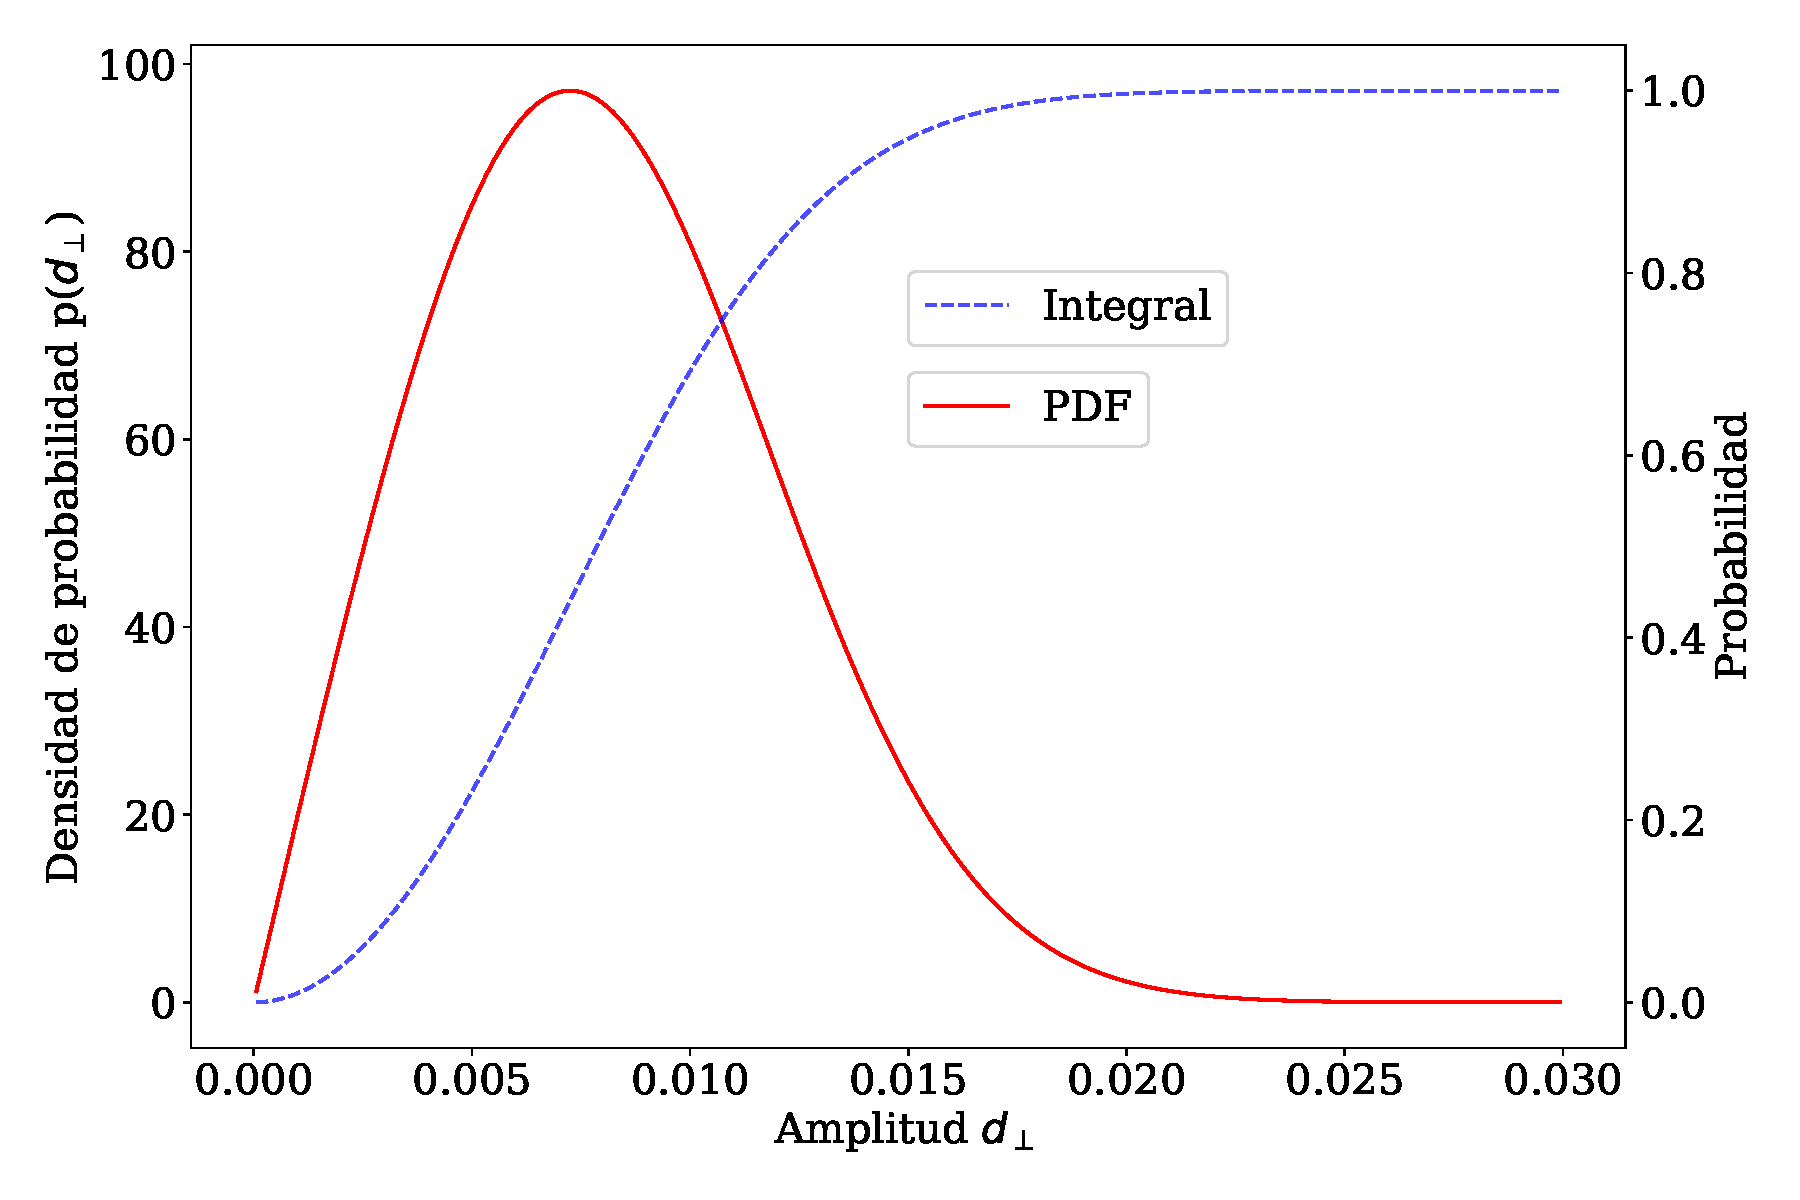
\includegraphics[width=0.75\textwidth]{bessel_prob.pdf}
        \end{center}
        \caption{}
    \end{small}
\end{figure}


\subsection{Haciendo la cuenta de los márgenes de confianza de la amplitud}

Los pasos que sigo son los siguientes: 

\begin{enumerate}
    \item Calculo la probabilidad asociada a $r_{max}=r +  10\sigma$. Dado que está tan alejada del valor de amplitud obtenida, el CL$\simeq 1$, por lo que uso este valor para normalizar  la Ec. \ref{ec:pdf} en el código.
    \item Una vez que tengo la función normalizada, finalmente hago la integral de la ecuación \ref{ec:integral} $CL(r)$ hasta un valor inicial de $r$ y el valor de la función $p(r)$.
    \begin{figure}[H]
        \begin{small}
            \begin{center}
                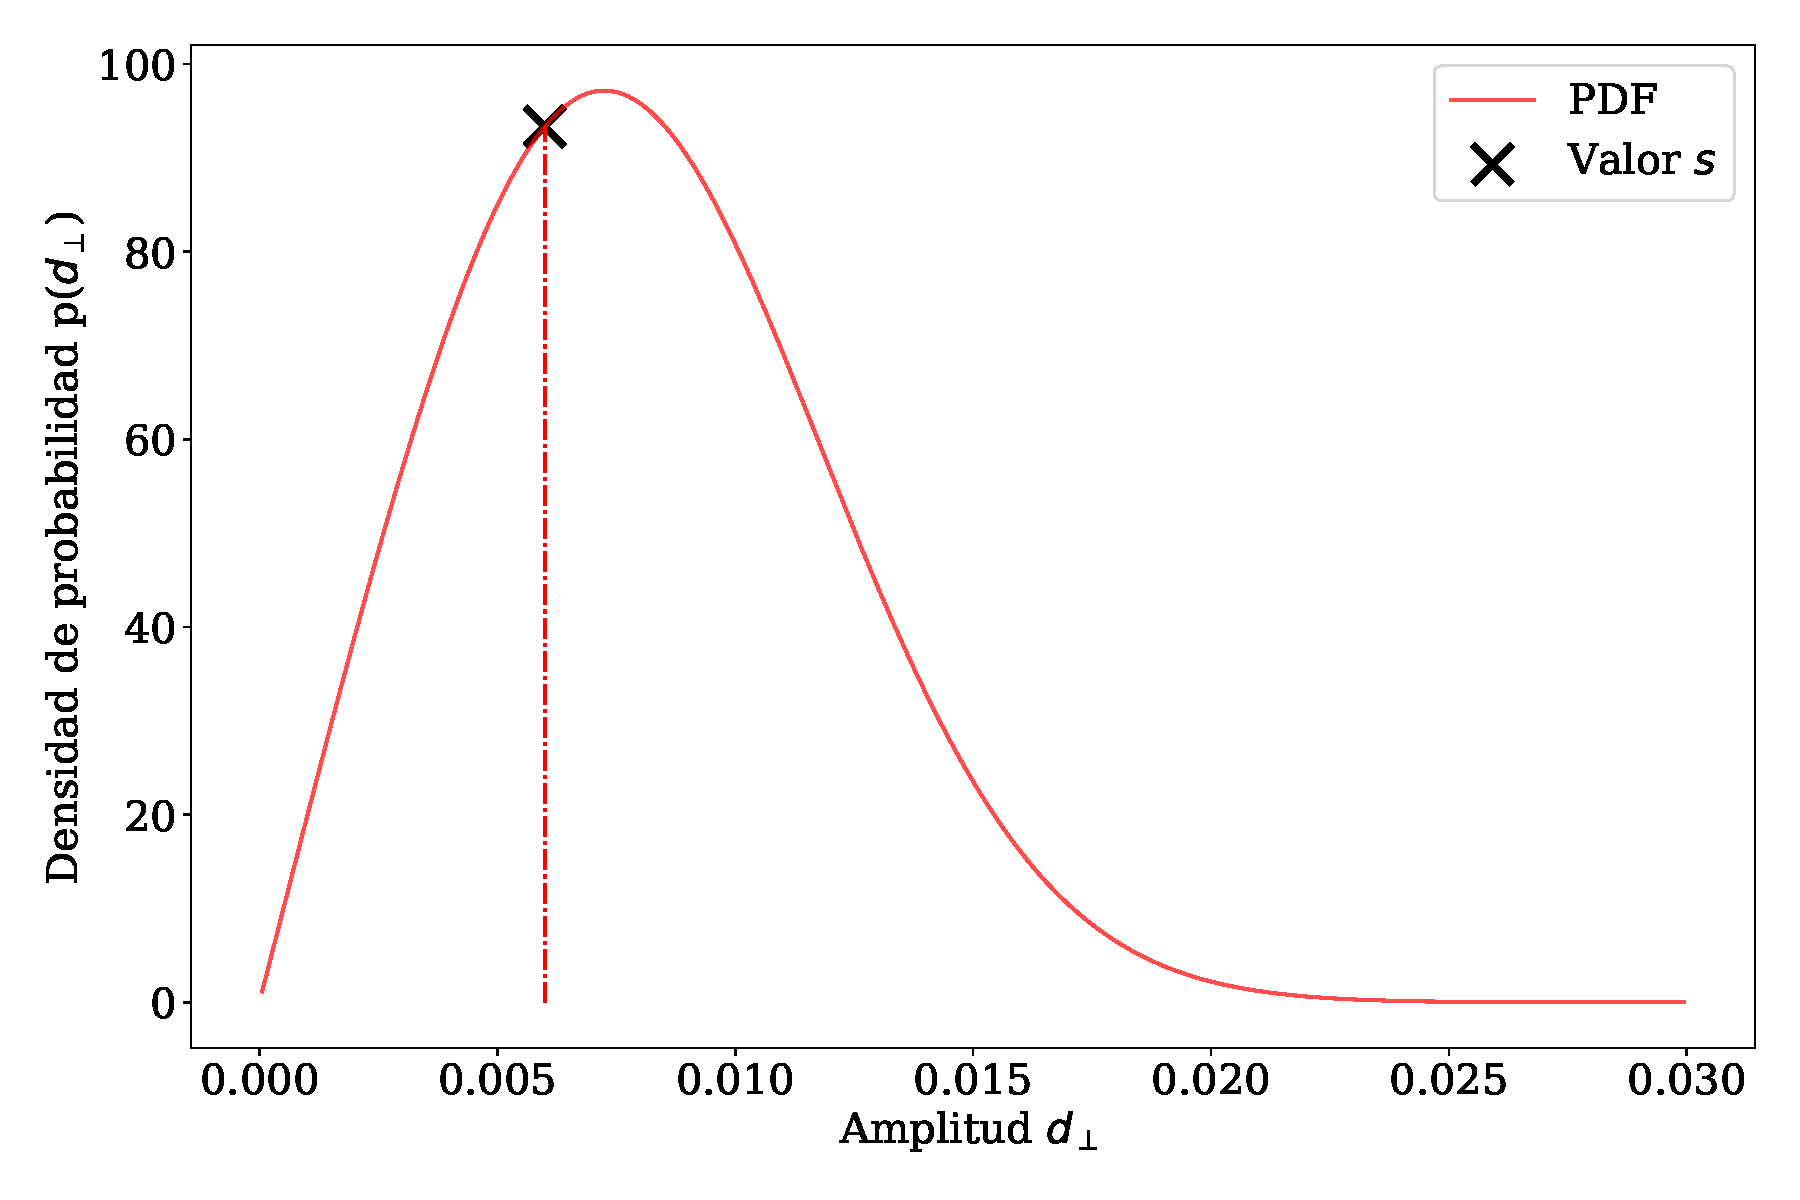
\includegraphics[width=0.75\textwidth]{bessel_prob_value_s.pdf}
            \end{center}
            \caption{}
        \end{small}
    \end{figure}
    \item Si $CL(r)< 0.683$:
    \begin{enumerate}
        \item Teniendo en cuenta el valor inicial de $p(r)_1$, se actualiza el valor  $p(r)_2 \leftarrow p(r)_1 - 0.01 p(r)_1$ \label{itm:1}.
        \item Se calcula la integral entre los dos puntos con valores igual a $p(r)_2$. 
        \item \label{itm:3} Si la integral es menor a $0.683$, se repite el proceso desde el paso \ref{itm:1}. Caso contrario, si esta integral es mayor o igual a $0.683$, se calculan los valores límites de $r$ mediante el valor $p(r)_2$ en el siguiente paso. 

        \begin{figure}[H]
            \begin{small}
                \begin{center}
                    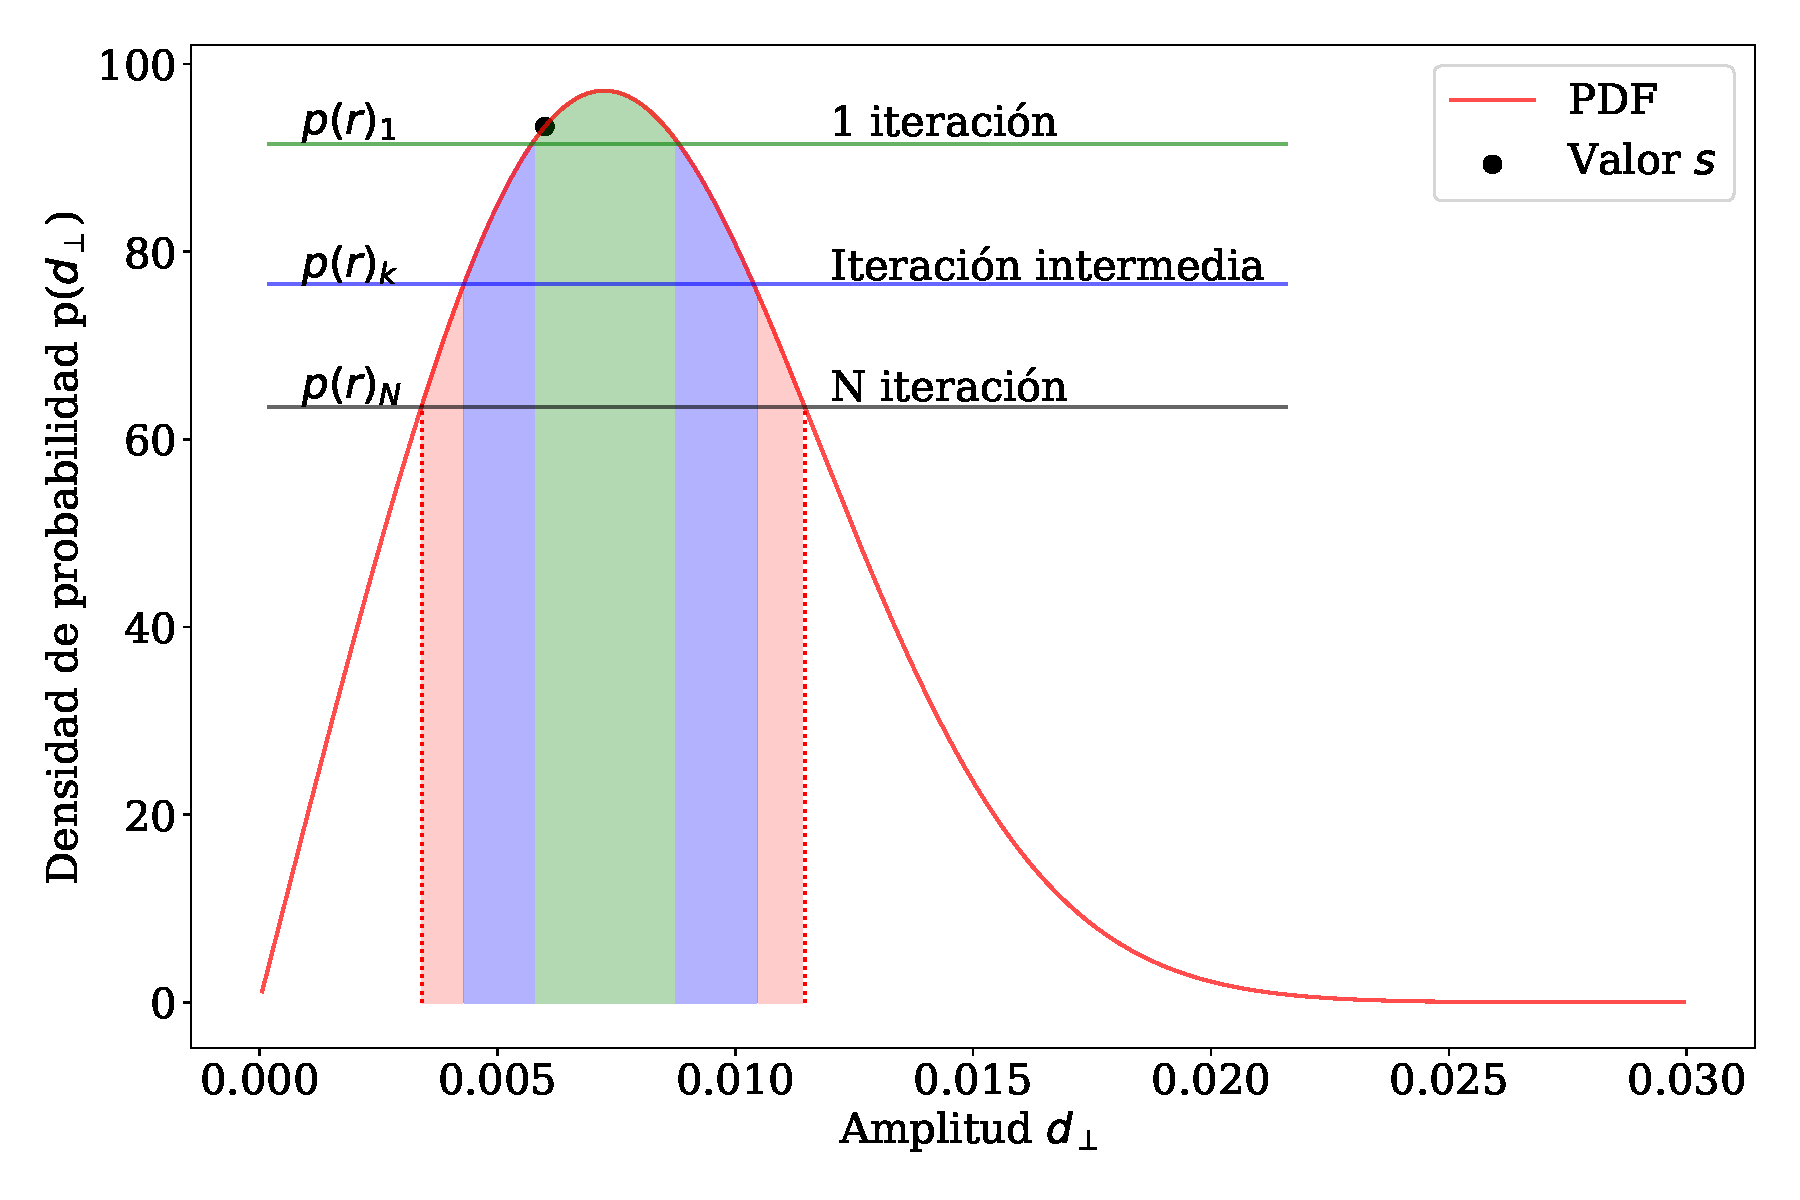
\includegraphics[width=0.75\textwidth]{bessel_prob_iterations.pdf}
                \end{center}
                \caption{}
            \end{small}
        \end{figure}



    \end{enumerate}
    \item Para calcular los límites de confianza superior $r^+$  y inferior $r^-$, teniendo en cuenta el valor final $p(r_N)$ del paso \ref{itm:3}, se calculan los valores de $r_i$ donde se cumple que $p(r_i)=p(r)_N$, los mismos son $r^+$  y  $r^-$. Finalmente los límites de confianza se calculan como:
    \begin{align*}
        \sigma^- = r-r^-\\
        \sigma^+ = r^+ -r
    \end{align*}
\end{enumerate}

\begin{figure}[H]
    \begin{small}
        \begin{center}
            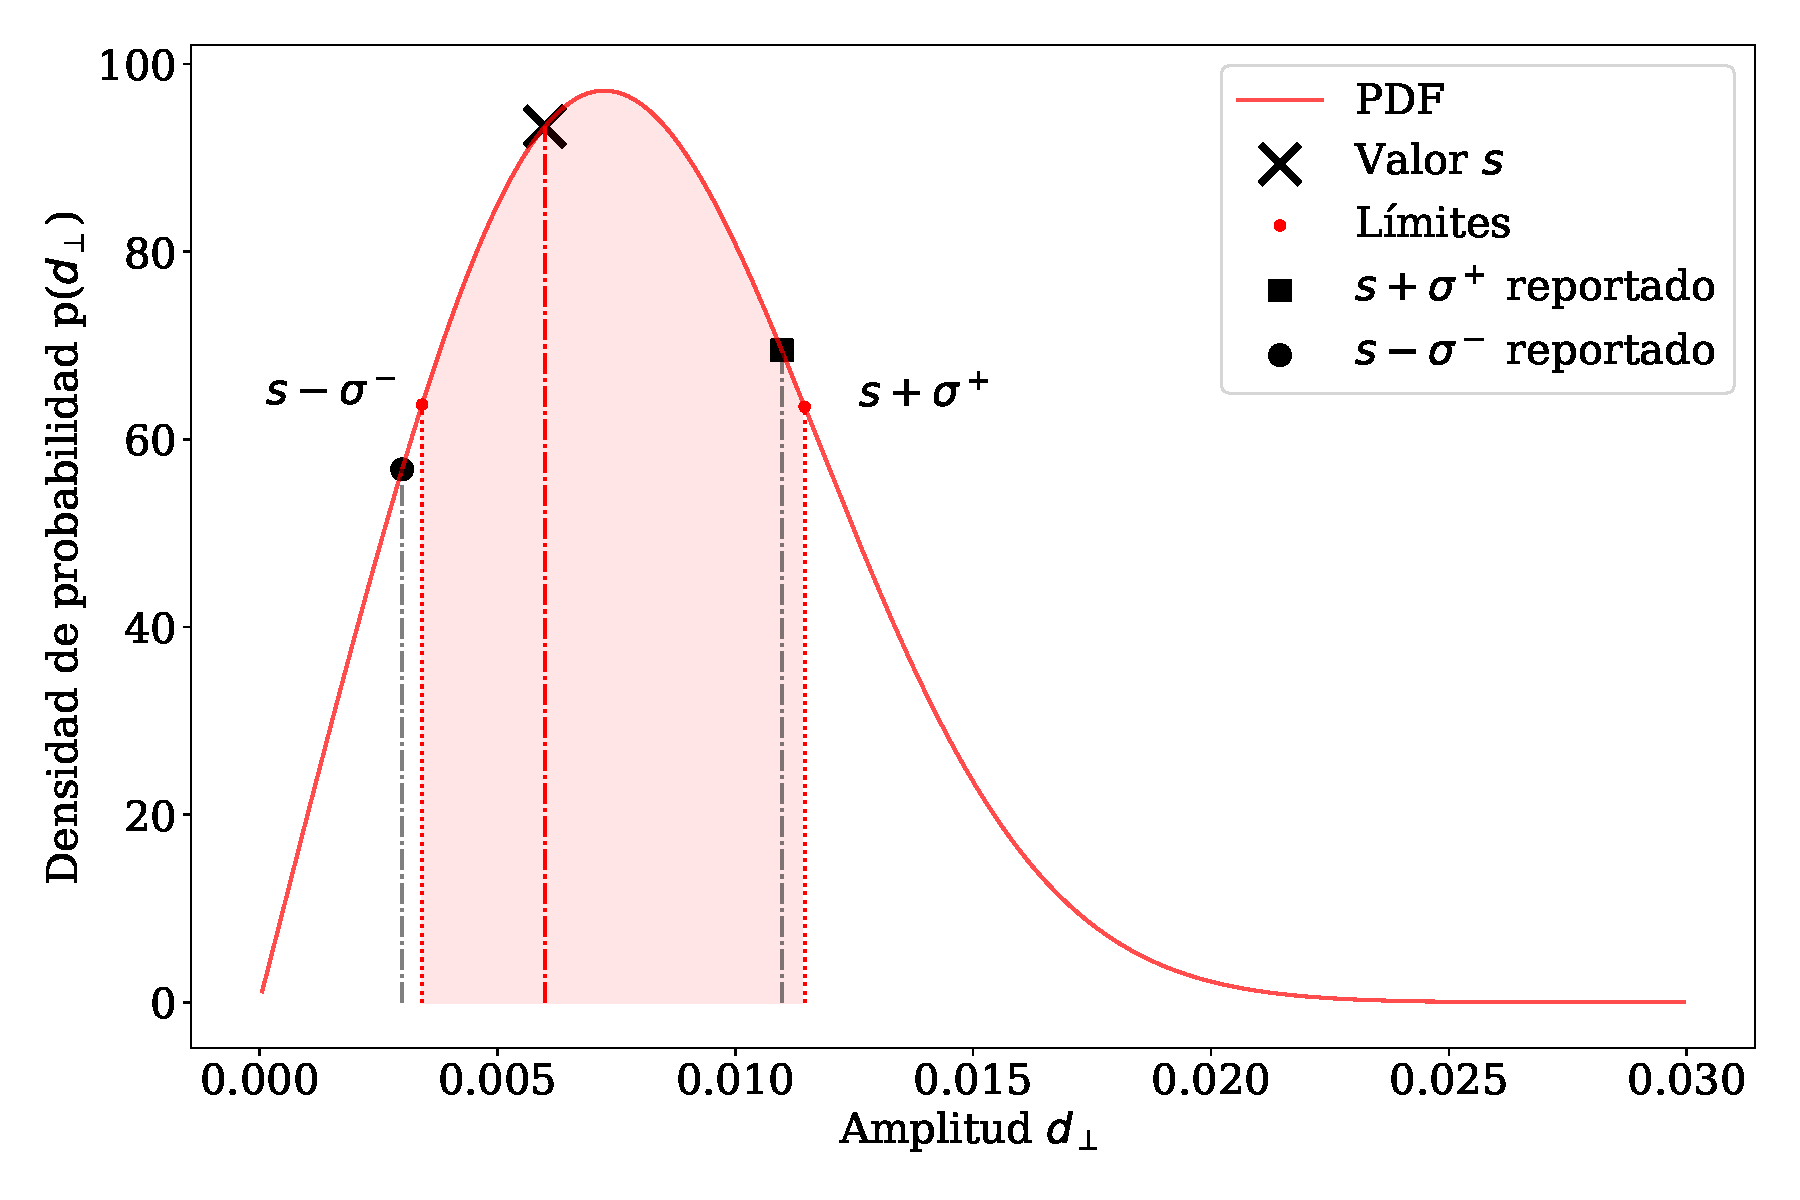
\includegraphics[width=0.75\textwidth]{bessel_prob_ej_0-25_0-5.pdf}
        \end{center}
        \caption{}
    \end{small}
\end{figure}


\section{Tabla cantidad de eventos para distintos rangos de energía}

Los eventos son clasificados en los distintos rangos con la energía reportada el archivo del Herald de todos los disparos  entre el 2014 y 2019 y para el disparo estándar entre el 2004 y 2018.


\begin{table}[H]
    \begin{small}
        \begin{center}
            \begin{tabular}{|l|l|l|l|l|}
                \hline
                \multicolumn{2}{|l|}{Rango}                                                          & 0.25 EeV- 0.5 EeV & 0.5 EeV - 1 EeV & 1 EeV - 2 EeV \\ \hline
                \multirow{2}{*}{Eventos}                                                  & Todos    & $3\,967\,368$     & $3\,638\,226$   & $1\,081\,846$ \\ \cline{2-5} 
                                                                                          & Estandar & $770\,323$        & $2\,388\,468$   & $1\,243\,098$ \\ \hline
                \multirow{2}{*}{\begin{tabular}[c]{@{}l@{}}Energía \\ Media\end{tabular}} & Todos    & $0.375$           & $0.687$         & $1.315$       \\ \cline{2-5} 
                                                                                          & Estandar & $0.42$            & $0.71$          & $1.34$.       \\ \hline
                \end{tabular}
            \caption{Tabla de eventos por rango de energía }
            \label{tab:}
        \end{center}
    \end{small}
\end{table}

\section{Resultados en distintos rangos de energía}
\subsection{Resultados en el rango 0.25 EeV - 0.5 EeV}

En la Fig. \ref{fig:primer} se comparan las direcciones en las que apuntan la fase en frecuencia sidérea obtenida en este trabajo con la obtenida en \cite{Aab_2020}. 
Las fases tiene un margen donde se solapan en la incertidumbre pero no son comparables, la línea punteada marca la dirección del centro galáctico.
\begin{table}[H]
    \begin{small}
        \begin{center}
            \begin{tabular}[c]{l|c||c|c}
                Frecuencia:                 & 365.25	  & 366.25	                    & 366.25 \cite{Aab_2020}   \\ 
                \hline
                Amplitud r [\%]:            & 0.17	      & $0.12^{+0.24}_{-0.03}$ 	    & $0.5^{+0.4}_{-0.2}$ \cite{codigo}      \\
                $r_{99}$ [\%]:              & 0.73	      & 0.6                         & 1.5\cite{codigo}                 \\
                $r^{UL}$ [\%]:              & - 	      & -                           & -\cite{codigo}                 \\
                \hline
                Amplitud $d_\perp$[\%]:     & -	          & $0.16^{+0.31}_{-0.04}$ 	    & $0.6^{+0.6}_{-0.3}$       \\
                $d_{99}$ [\%]:              & - 	      & -                           & -                 \\
                $d_{\perp,UL}$[\%]:         & -           & 0.8       & 1.8      \\
                \hline
                $\sigma_{x,y}$[\%]:         & -	          & 0.24	   & 0.48       \\
                Probabilidad      :         & 0.66        & 0.81	   & 0.45       \\
                Fase[$^o$]:                 & 221$\pm$63  & 280$\pm$88 & 225$\pm$64\cite{discrepancia} \\
            \end{tabular}
        \end{center}
    \end{small}
    \caption{Características para las frecuencias solar y sidérea con el método East-West en el primer armónico en rango de energía 0.25 EeV - 0.5 EeV}
    \label{tab:solar}
\end{table}


Realizando el barrido de frecuencias con la variable de la Ec.\ref{ra_arb}, se obtiene que en este rango de energía las amplitudes se  distribuyen en frecuencia como se muestra en la Fig.\ref{fig:primer_barrido}. La línea horizontal indica el valor de $r_{99}$ para cada frecuencia, además se observa que ninguna frecuencia supera dicho umbral.

\begin{figure}[H]
    \begin{small}
        \begin{center}
            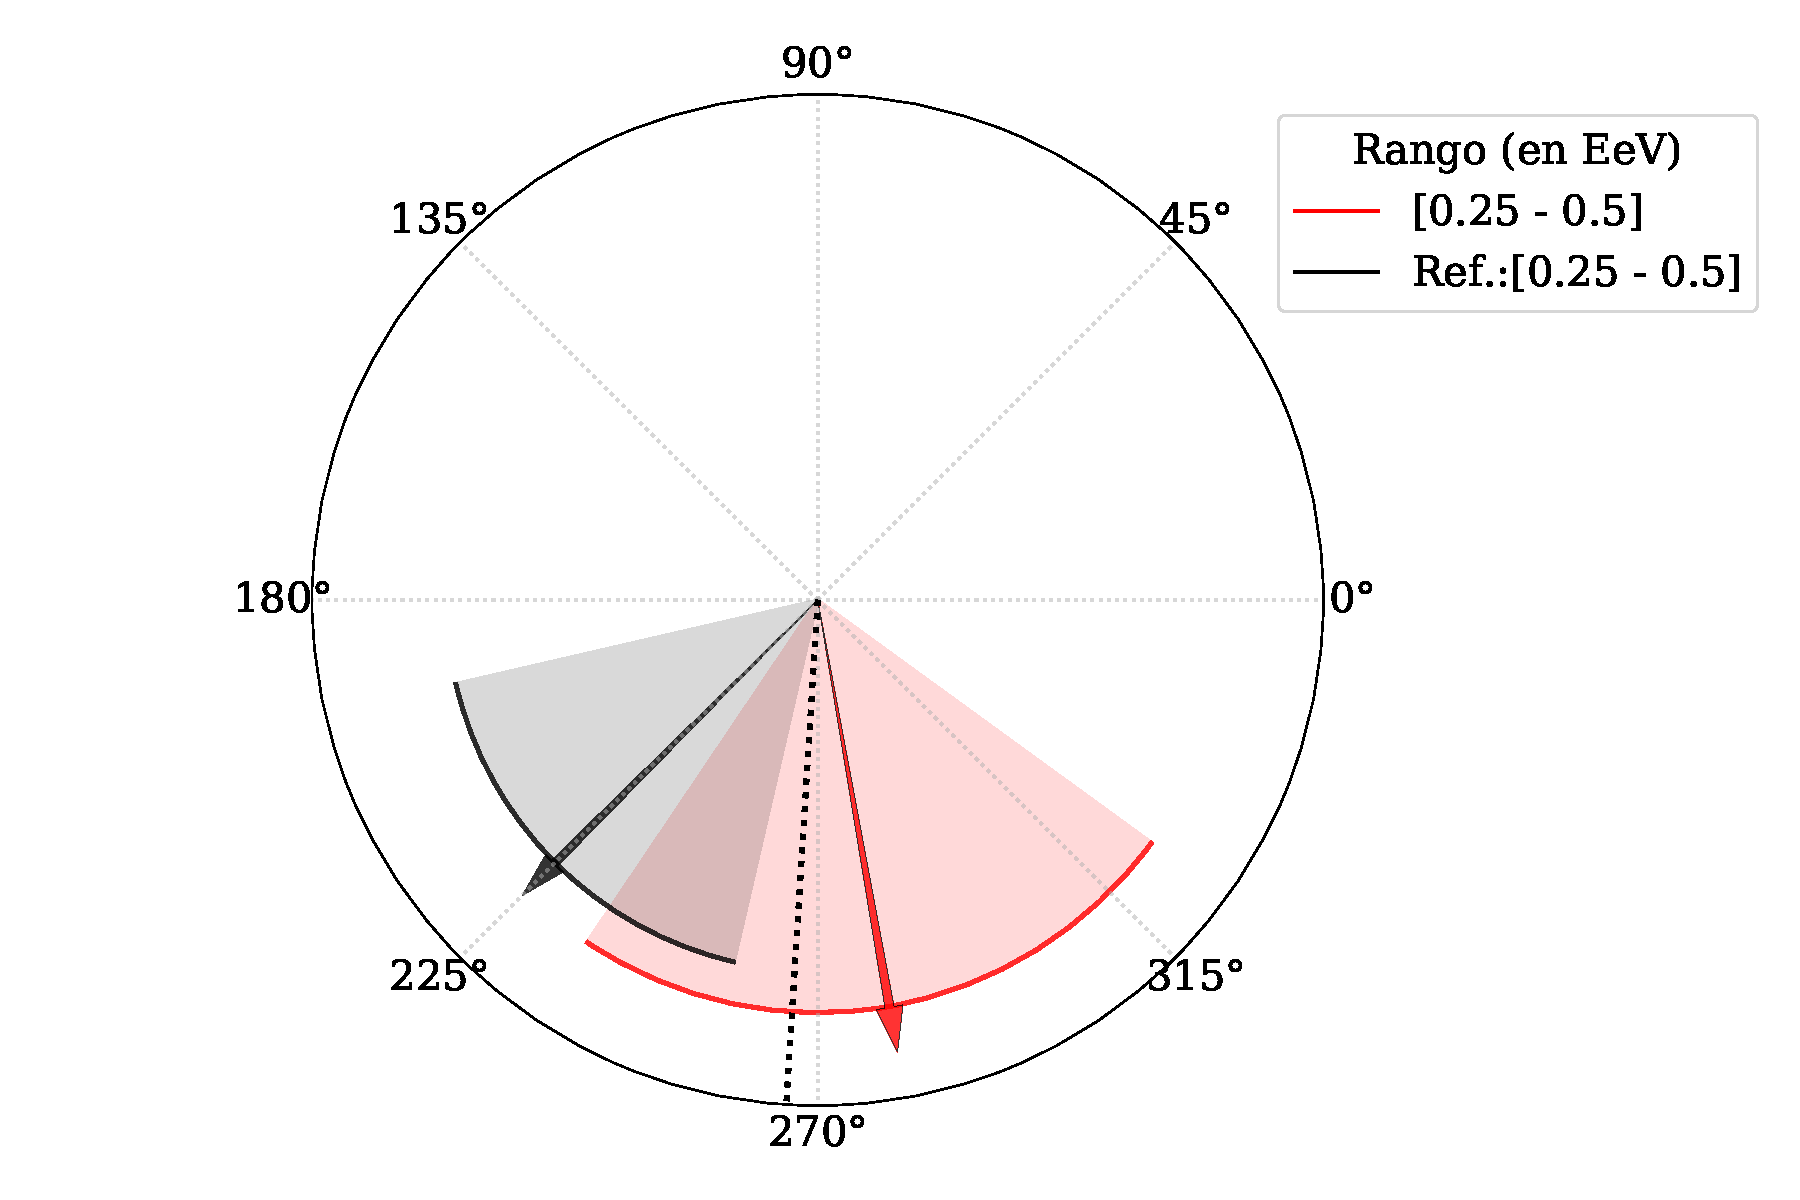
\includegraphics[width=0.75\textwidth]{phase_primer_bin.pdf}
        \end{center}
        \caption{Valores de las fases obtenidos en este trabajo y en la referencia con sus respectivas incertidumbres para la frecuencia sidérea en el  rango 0.25 EeV - 0.5 EeV .}
        \label{fig:primer}
    \end{small}
\end{figure}

\begin{figure}[H]
    \begin{small}
        \begin{center}
            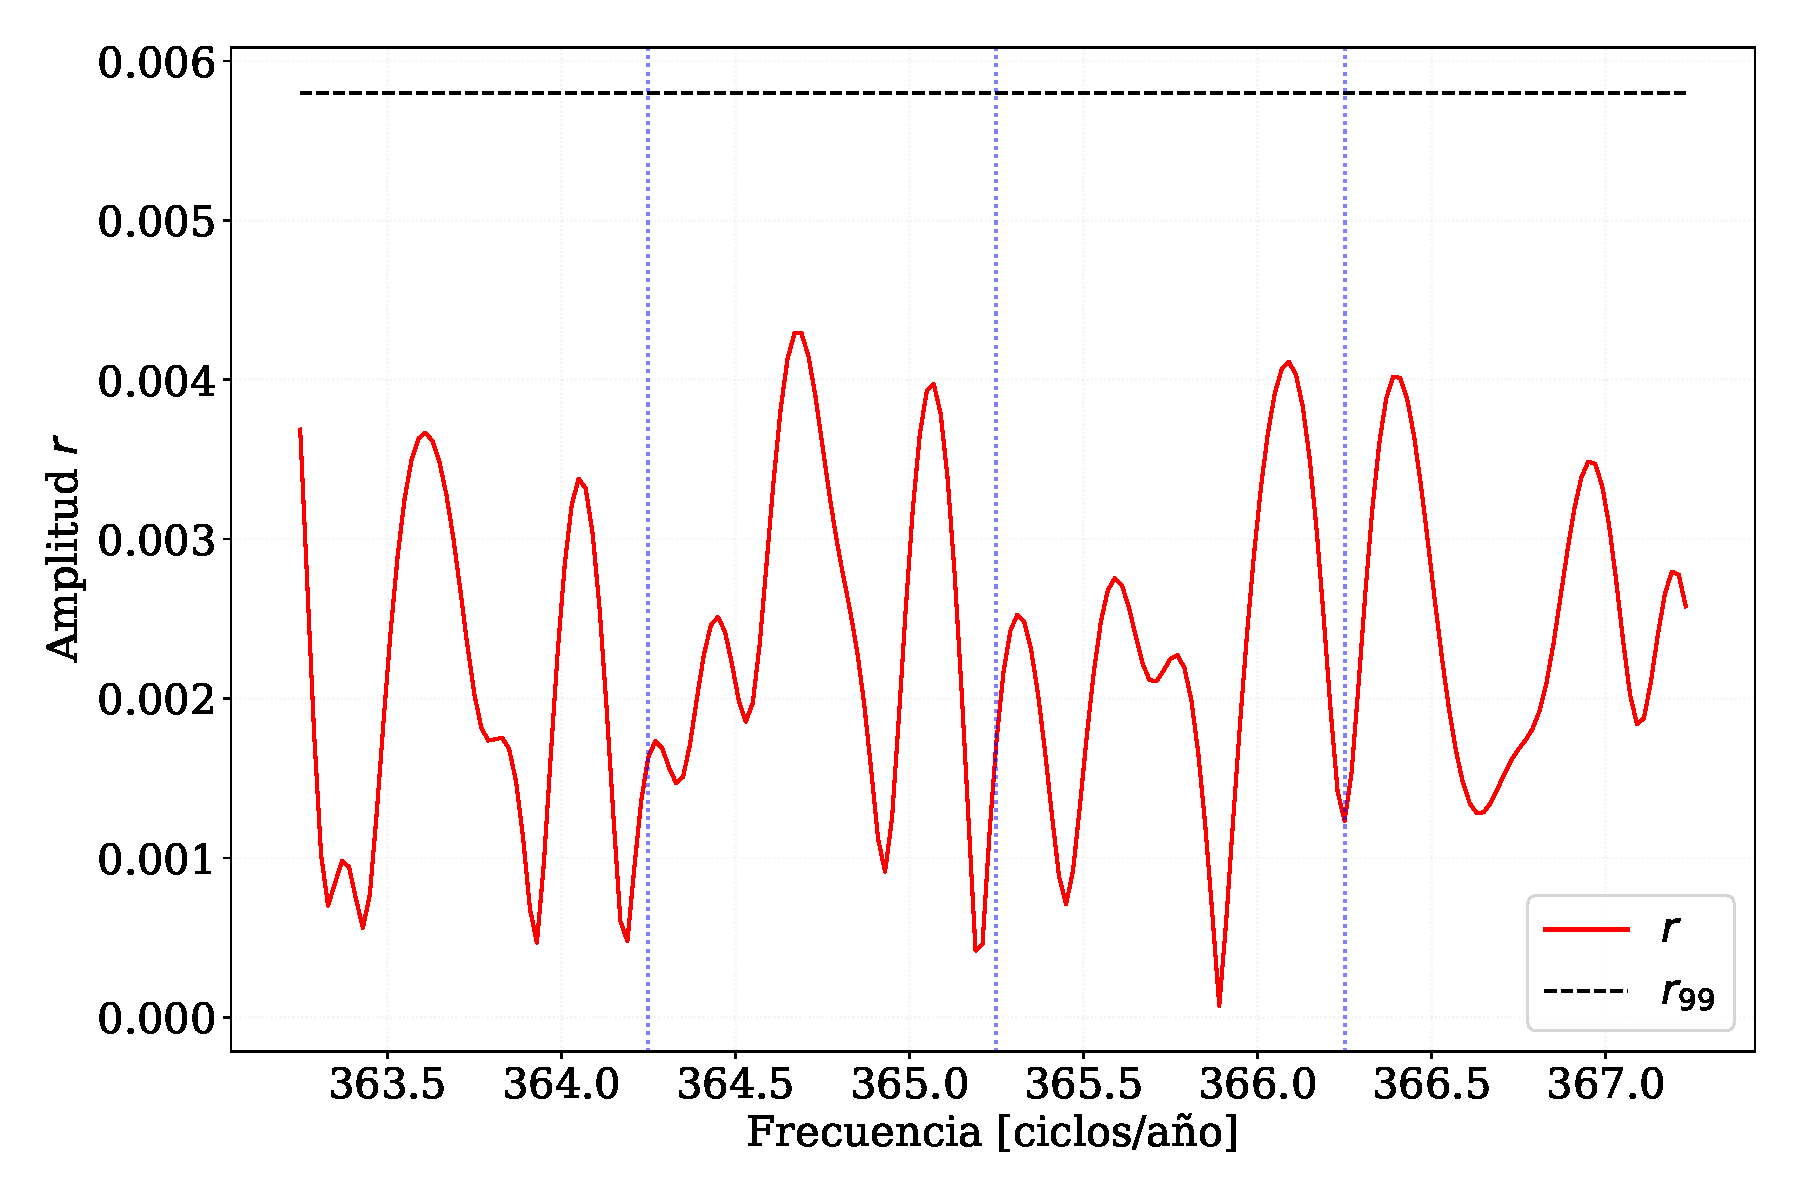
\includegraphics[width=0.75\textwidth]{plot_bin_1_barrido_v2.pdf}
        \end{center}
        \caption{Barrido de frecuencias en el  rango 0.25 EeV - 0.50 EeV .}
        \label{fig:primer_barrido}
    \end{small}
\end{figure}

\subsection{Resultados en el rango 0.5 EeV - 1 EeV}
En este rango de energía se observa una diferencia entre las probabilidades de este trabajo y \cite{Aab_2020}  ne la frecuencia sidérea. Este valor dice cuando probable es que las amplitudes sean debido al ruido. Este trabajo obtiene que la amplitud en sidérea es significativa por un  $6\%$.  

En la Fig. \ref{fig:segundo} se comparan las direcciones en las que apuntan la fase en frecuencia sidérea obtenida en este trabajo con la obtenida en \cite{Aab_2020}. En esta figura se observa que las fases son comparables entre sí y apuntan a una dirección cercana al centro galáctico (línea punteada).

El barrido de frecuencias con la variable de la Ec.\ref{ra_arb} para este rango de energía se observa en la Fig.\ref{fig:segundo_barrido}. La línea horizontal indica el valor de $r_{99}$ para cada frecuencia, además se observa que ninguna frecuencia supera dicho umbral. Otro aspecto es que la zona de la frecuencia anti-sidérea no tiene picos pronunciados, como en la frecuencia solar o sidérea.

\begin{figure}[H]
    \begin{small}
        \begin{center}
            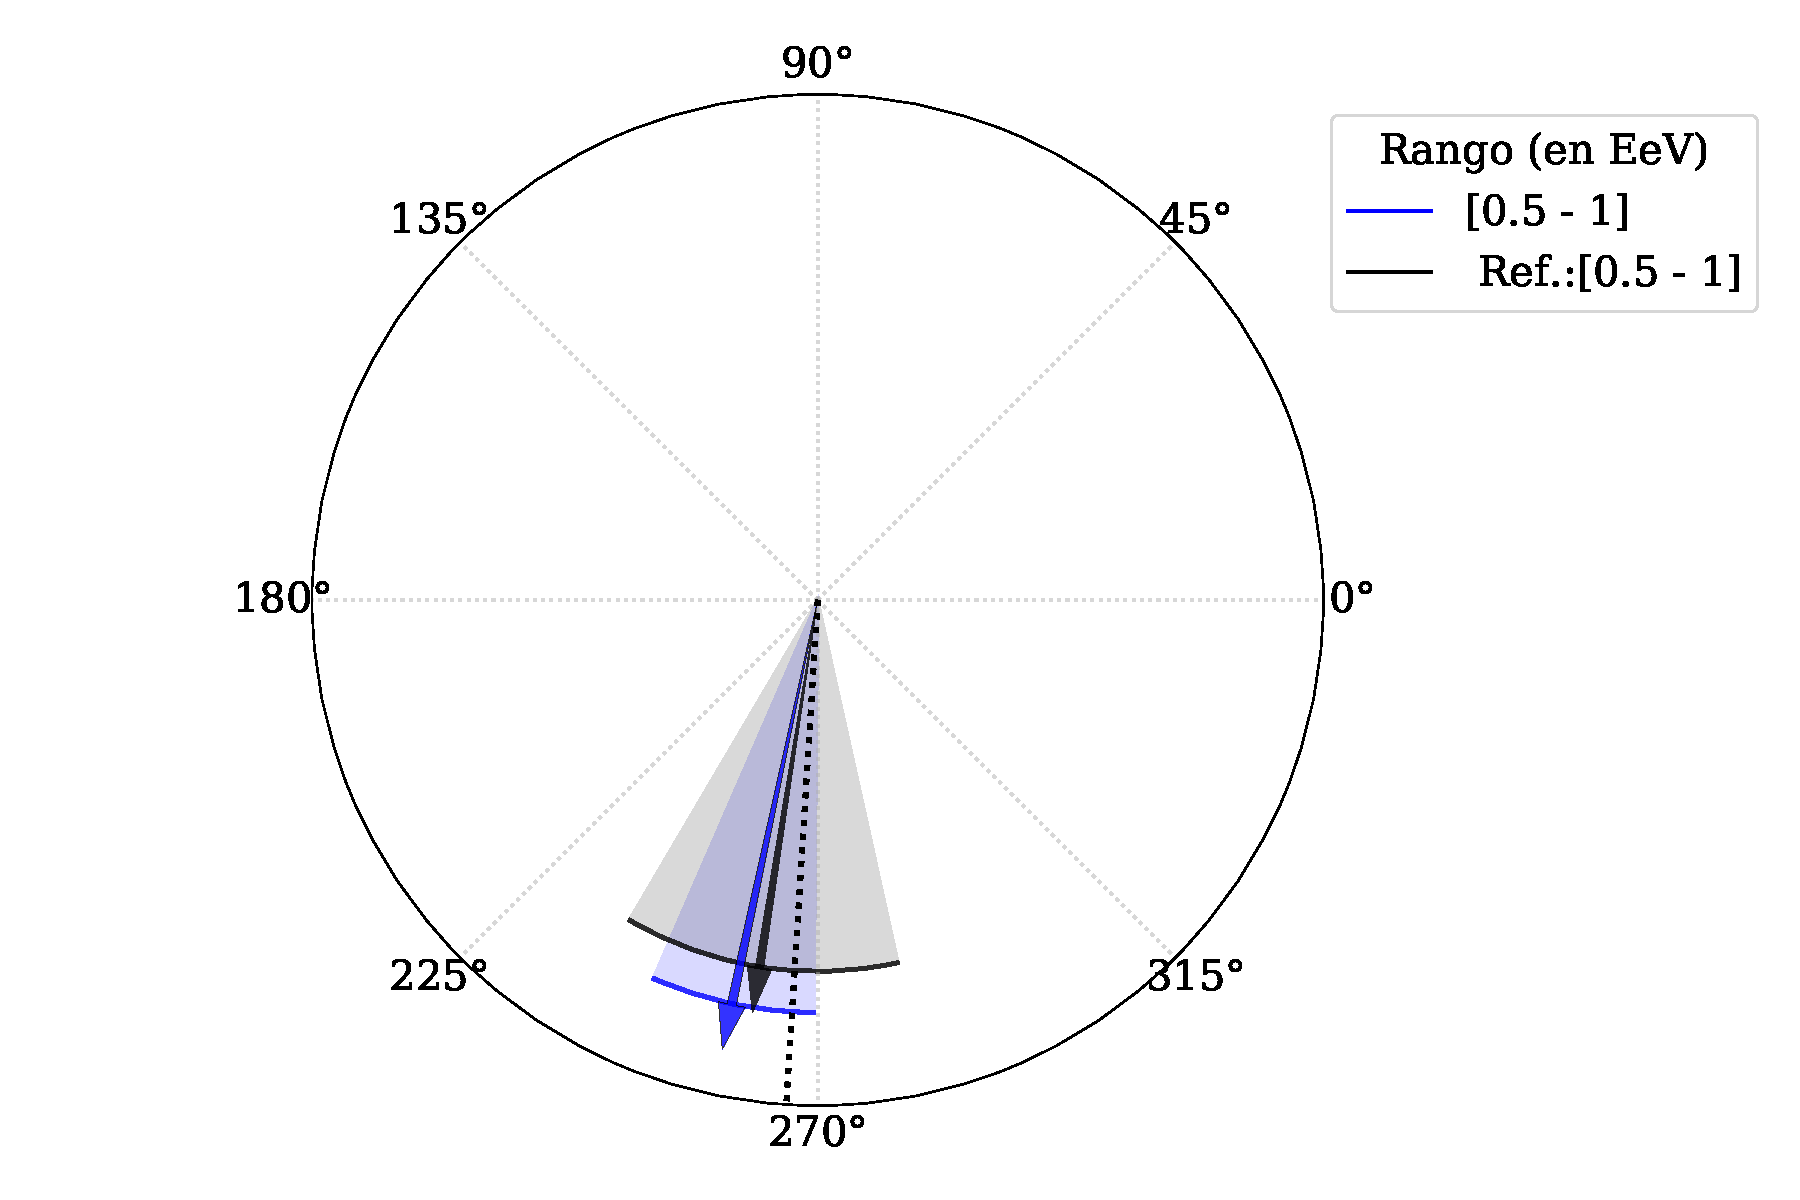
\includegraphics[width=0.75\textwidth]{phase_segundo_bin.pdf}
        \end{center}
        \caption{Valores de las fases obtenidos en este trabajo y en la referencia con sus respectivas incertidumbres para la frecuencia sidérea en el  rango 0.5 EeV - 1.0 EeV .}
        \label{fig:segundo}
    \end{small}
\end{figure}

\begin{table}[H]
        \begin{small}
            \begin{center}
                \begin{tabular}[c]{l|c||c|c}
                    Frecuencia:             & 365.25	    & 366.25		& 366.25\cite{Aab_2020}\\
                    \hline
                    Amplitud r [\%]:        & 0.42          & $0.4^{+0.2}_{-0.1}$ 	        & $0.40^{+0.2}_{-0.1}$\cite{codigo}  \\
                    $r_{99}$[\%]:           & 0.70	        & 0.6          & 0.8\cite{codigo}  \\
                    $d_{\perp,UL}[\%]$      & -             & 1.1          & 1.1\\                    
                    \hline
                    Amplitud $d_\perp$[\%]: & -             & $0.6^{+0.3}_{-0.2}$           & $0.50^{+0.3}_{-0.2}$\\
                    $r_{99}$[\%]:           & 0.70	        & 0.6          & 0.8\cite{codigo}  \\
                    $d_{\perp,UL}[\%]$      & -             & 1.1          & 1.1\\

                    $\sigma_{x,y}$[\%]:     & -	            & 0.23	        & 0.27       \\
                    Probabilidad:           & 0.06          & 0.06	        & 0.20\\
                    Fase[$^o$]:             & 205$\pm$25	& 258$\pm$24	& 261$\pm$43\cite{discrepancia}   \\
                \end{tabular}
            \end{center}
        \end{small}
        \caption{Características para las frecuencias solar y sidérea con el método East-West en el primer armónico en rango de energía 0.5 EeV - 1 EeV}
        \label{tab:solar}
    \end{table}


    \begin{figure}[H]
        \begin{small}
            \begin{center}
                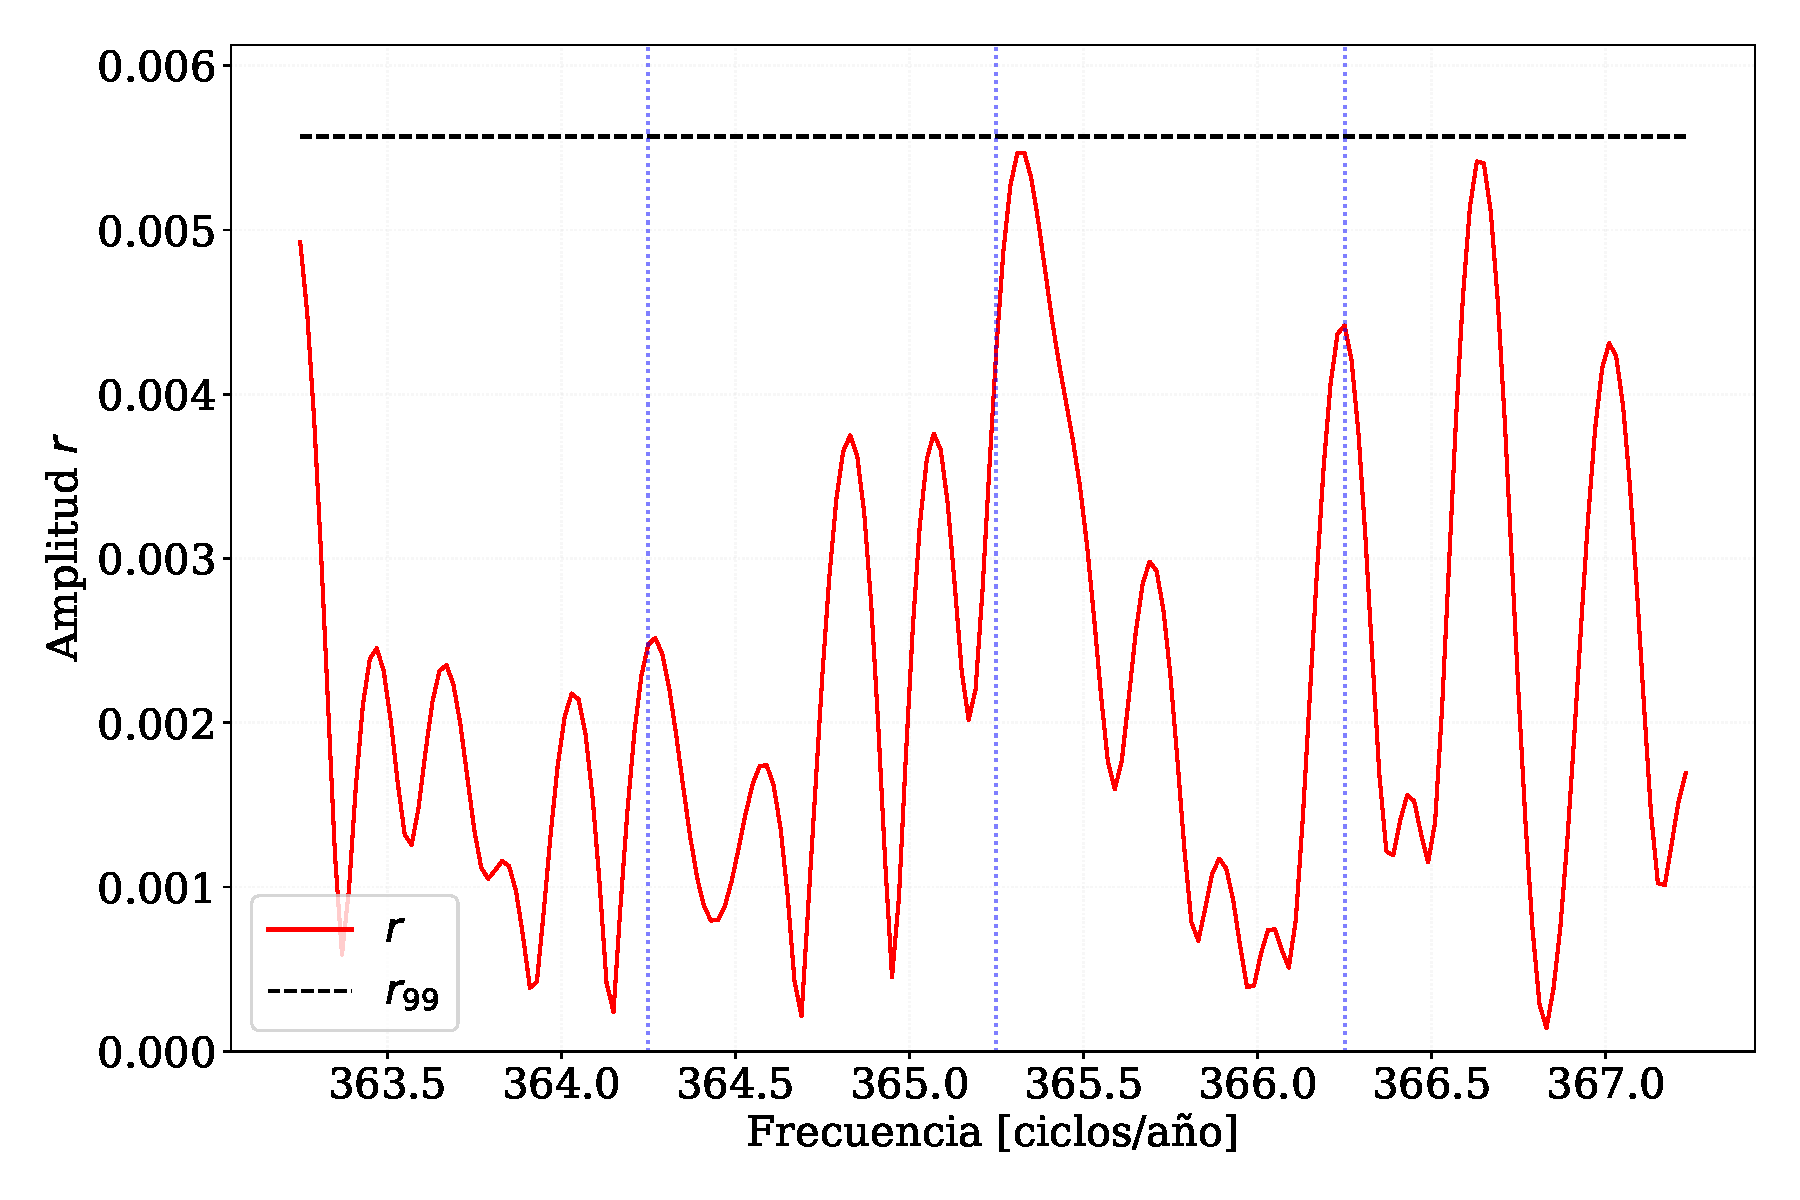
\includegraphics[width=0.75\textwidth]{plot_bin_2_barrido_v2.pdf}
            \end{center}
            \caption{Barrido de frecuencias en el  rango 0.5 EeV - 1.0 EeV .}
            \label{fig:segundo_barrido}
        \end{small}
    \end{figure}    


\subsection{Resultados en el rango 1 EeV - 2 EeV}

 
En las Tablas \ref{tab:solar_3} y \ref{tab:siderea_3} se comparan los resultados de este trabajo y los obtenidos en \cite{Aab_2020} para la frecuencia solar y sidérea respectivamente. En el Fig.\ref{fig:tercer} se observan en un gráfico polar las fases de la referencia y este trabajo para la frecuencia sidérea. Los resultados son comparables entre sí.
    
    \begin{table}[H]
        \begin{small}
            \begin{center}
                \begin{tabular}[c]{l|c|c}
                                    & Rayleigh      & EW            \\\hline
                    Frecuencia:     & 365.25	    & 365.25        \\
                    Amplitud $r$  [\%]:  & 0.39     & 0.28     \\
                    Probabilidad:   & 0.02          & 0.64          \\
                    Fase:           & 288$\pm$20    & 279$\pm$61    \\
                    $r_{99}$ [\%]:  & 0.41263       & 1.2       \\
                \end{tabular}
            \end{center}
        \end{small}
        \caption{Características para la frecuencia solar con los métodos de Rayleigh  e East-West en el primer armónico.}
        \label{tab:solar_3}
    \end{table}

    \begin{table}[H]
        \begin{small}
            \begin{center}
                \begin{tabular}[c]{l|c||c|c}
                                            & Rayleigh    & EW                          & EW\cite{Aab_2020}      \\\hline
                    Frecuencia:             & 366.25	  & 366.25                      & 366.25        \\
                    Amplitud $r$ [\%]:      & 0.40	      & $0.5^{+0.3}_{-0.2}$         & $0.14^{+0.37}_{-0.02}$\cite{codigo}       \\
                    Amplitud $d_\perp$ [\%]:& 0.51        & $0.6^{+0.4}_{-0.3}$         & $0.18^{+0.47}_{-0.02}$       \\ 
                    $\sigma_{x,y}$[\%]:     & -	          & 0.38	                    & 0.35          \\
                    Probabilidad:           & 0.012	      & 0.26                        & 0.87          \\
                    Fase[$^o$]:             & 330$\pm$20  & 320$\pm$30                  & 291$\pm$100 \cite{discrepancia}      \\
                    $r_{99}$[\%]:           & 0.41	      & 0.9                         & 0.84\cite{codigo}        \\
                    $d_{\perp,UL}[\%]$      & 0.53        & 1.6                         & 1.1        \\
                \end{tabular}
            \end{center}
        \end{small}
        \caption{Características para la frecuencia sidérea con los métodos de Rayleigh  e East-West en el primer armónico.}
        \label{tab:siderea_3}
    \end{table}
   
    \begin{figure}[H]
        \begin{small}
            \begin{center}
                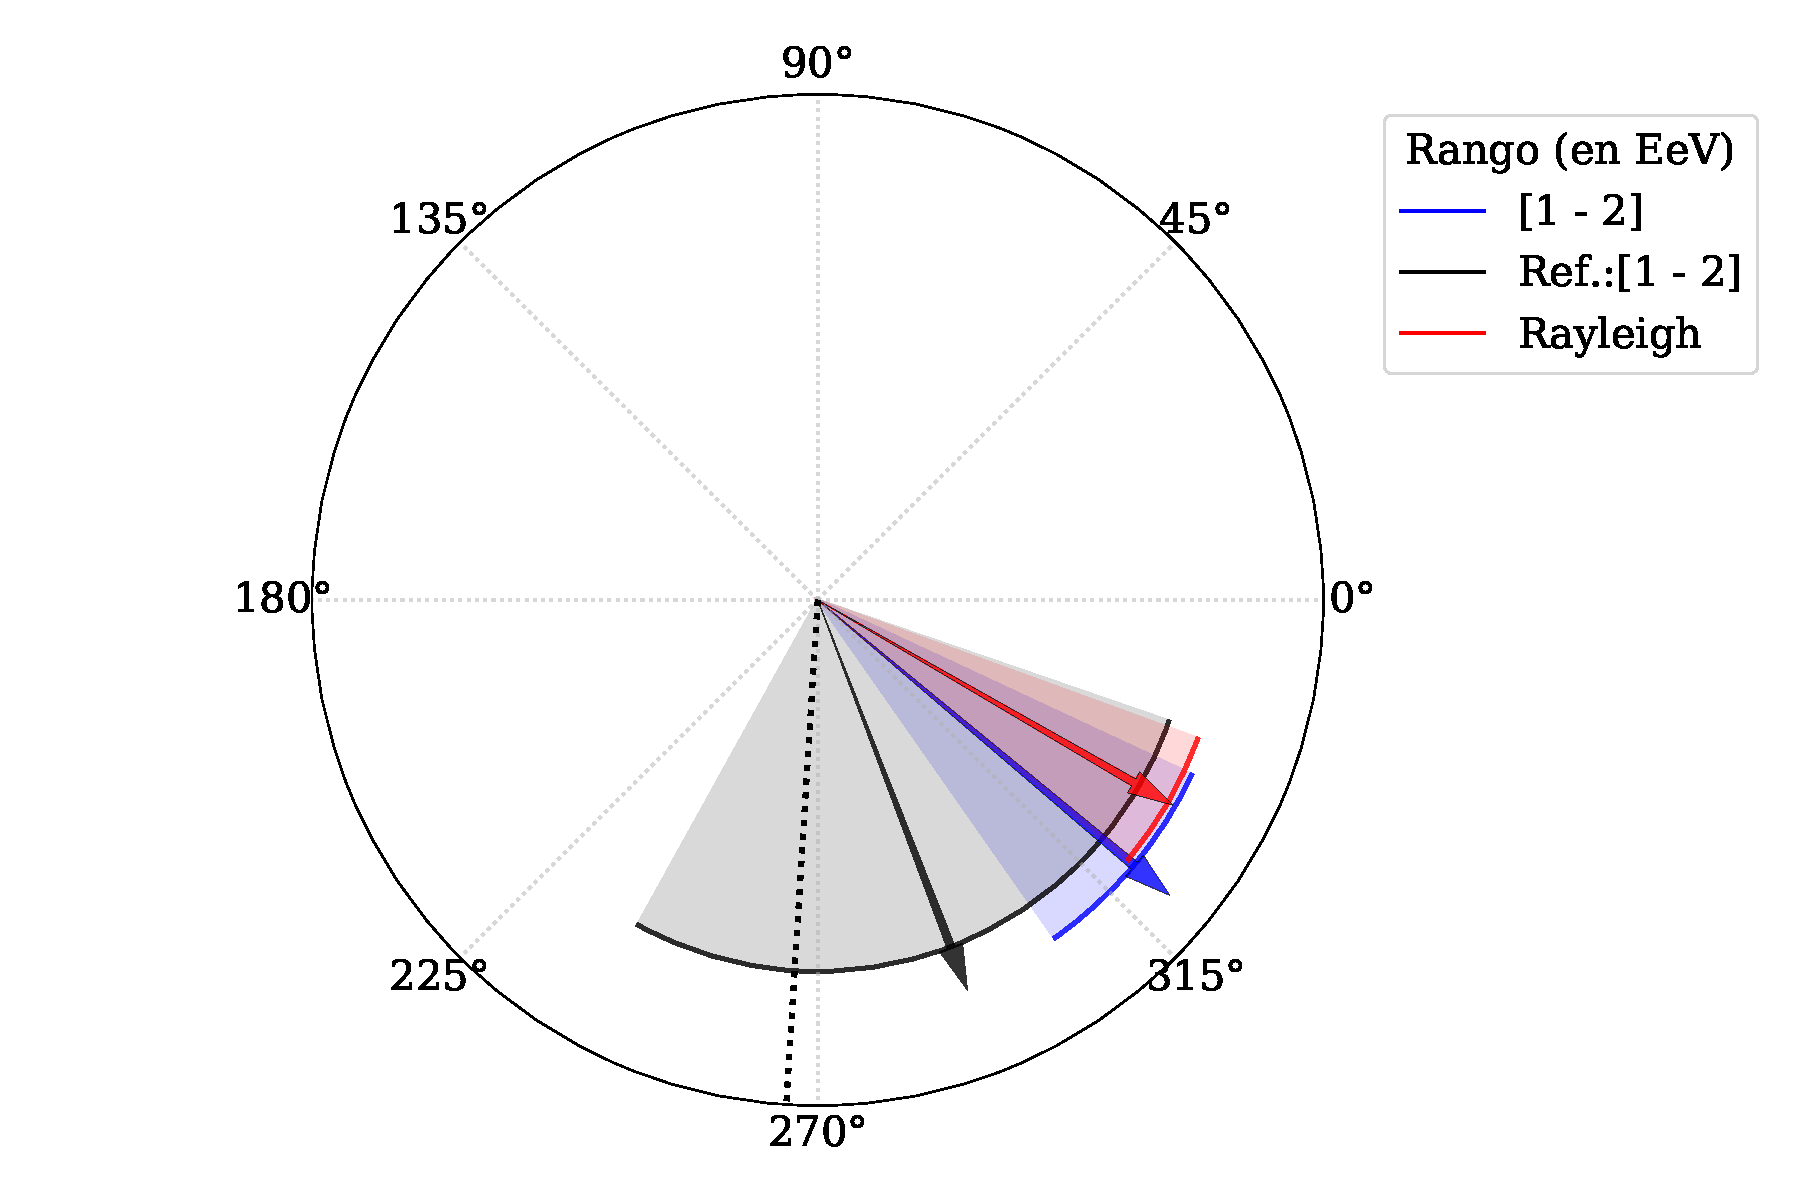
\includegraphics[width=0.75\textwidth]{phase_tercer_bin.pdf}
            \end{center}
        \caption{Valores de las fases obtenidos en este trabajo y en la referencia con sus respectivas incertidumbres para la frecuencia sidérea en el  rango 1.0 EeV - 2.0 EeV .}
        \label{fig:tercer}
        \end{small}
    \end{figure}


    El barrido de frecuencias con la variable de la Ec.\ref{ra_arb} para este rango de energía se observa en la Fig.\ref{fig:tercer_barrido}. La línea horizontal indica el valor de $r_{99}$ para cada frecuencia y se observa que ninguna frecuencia supera dicho umbral. En la frecuencia solar no se observa ningún pico, esto se debe a que el método EW es robusto con respecto a las modulación del clima. Se observa un pico en sidérea pero el mismo no es significativo con respecto al $r_{99}$.


    \begin{figure}[H]
        \begin{small}
            \begin{center}
                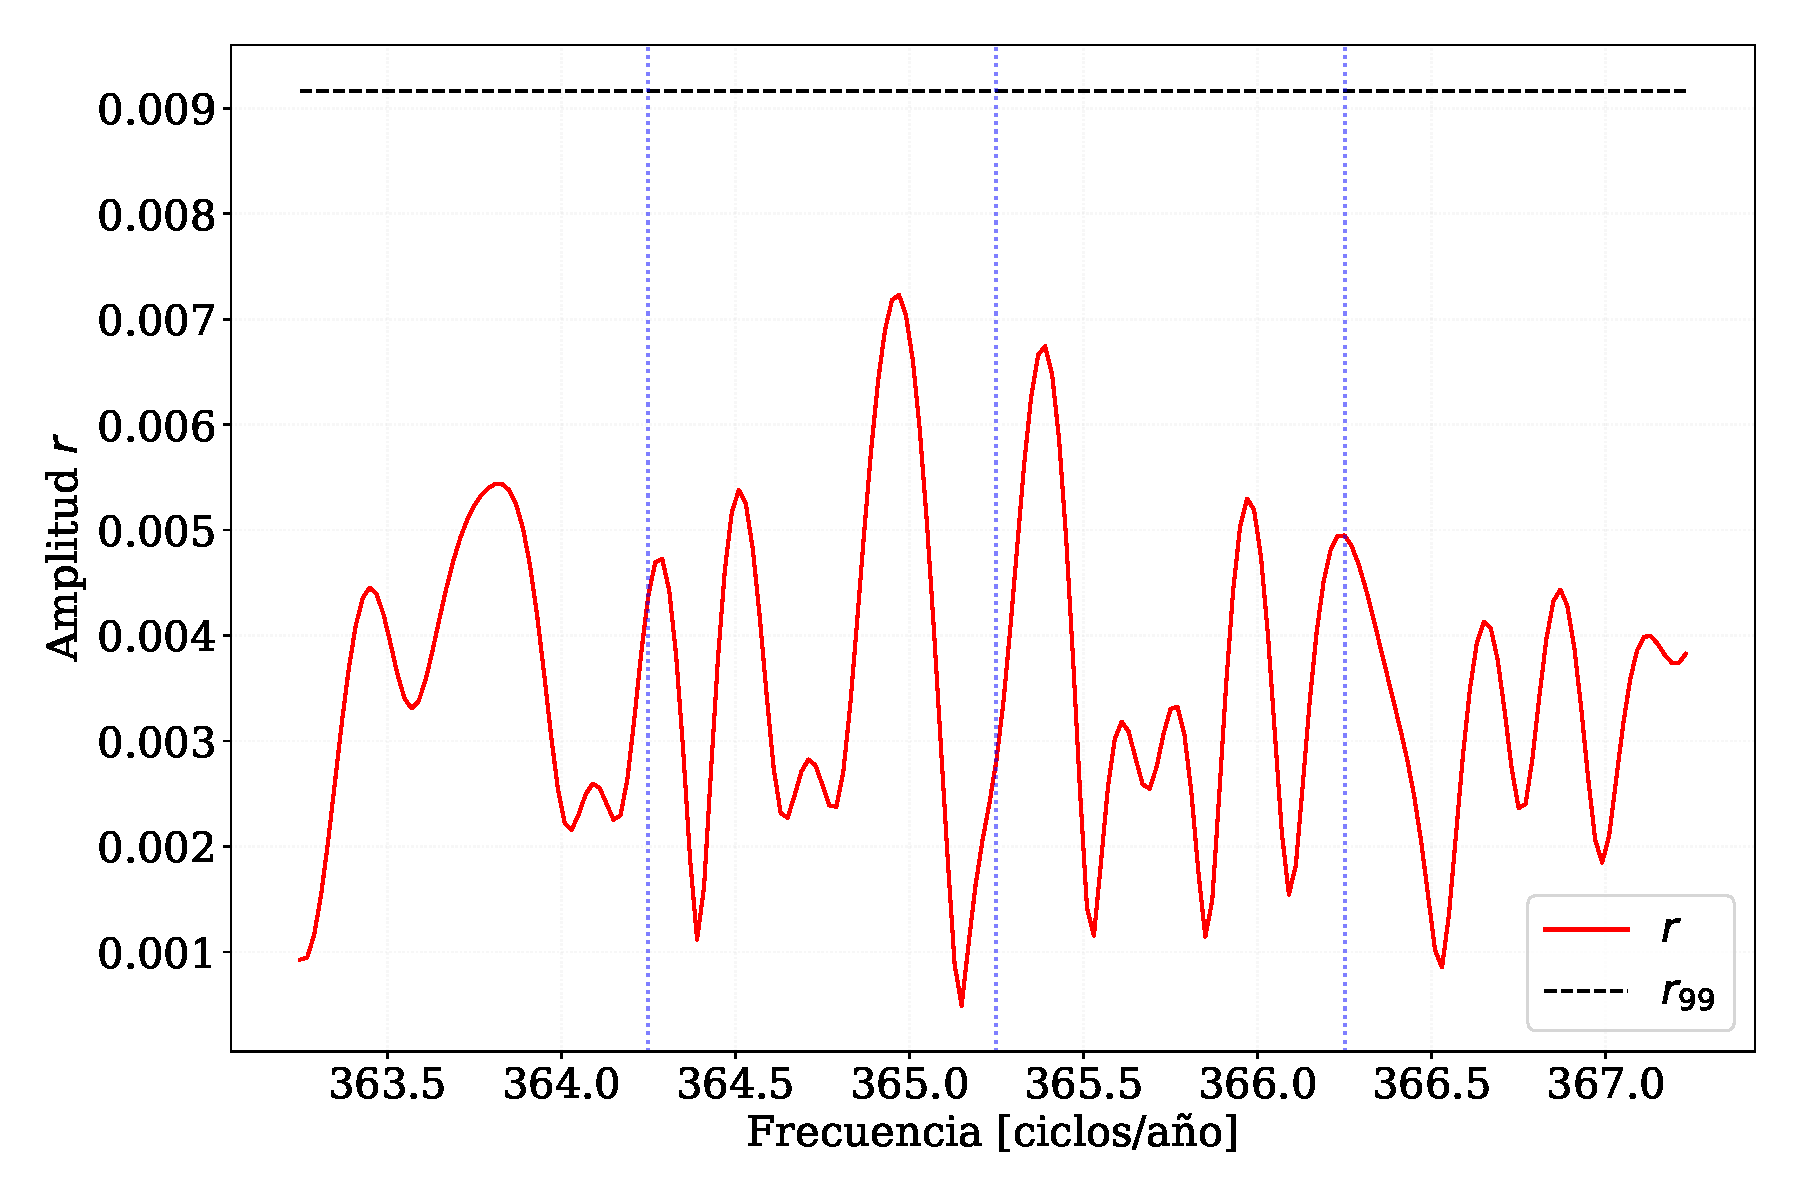
\includegraphics[width=0.75\textwidth]{plot_bin_3_barrido_v2.pdf}
            \end{center}
            \caption{Barrido de frecuencias en el rango 1 EeV - 2 EeV .}
            \label{fig:tercer_barrido}
        \end{small}
    \end{figure}    

    \section{Gráficos}

    Para poder comparar los resultados de $d_\perp$ entre sí, podríamos graficar los valores de la proyección y de la límite del $99\%$ como se muestra en la Fig.\ref{fig:no_normalizado}. El inconveniente es la cantidad de datos en cada rango de energía entre los conjuntos de datos, todos los disparos y disparo estándar, son distintos.



    \begin{figure}[H]
        \begin{small}
            \begin{center}
                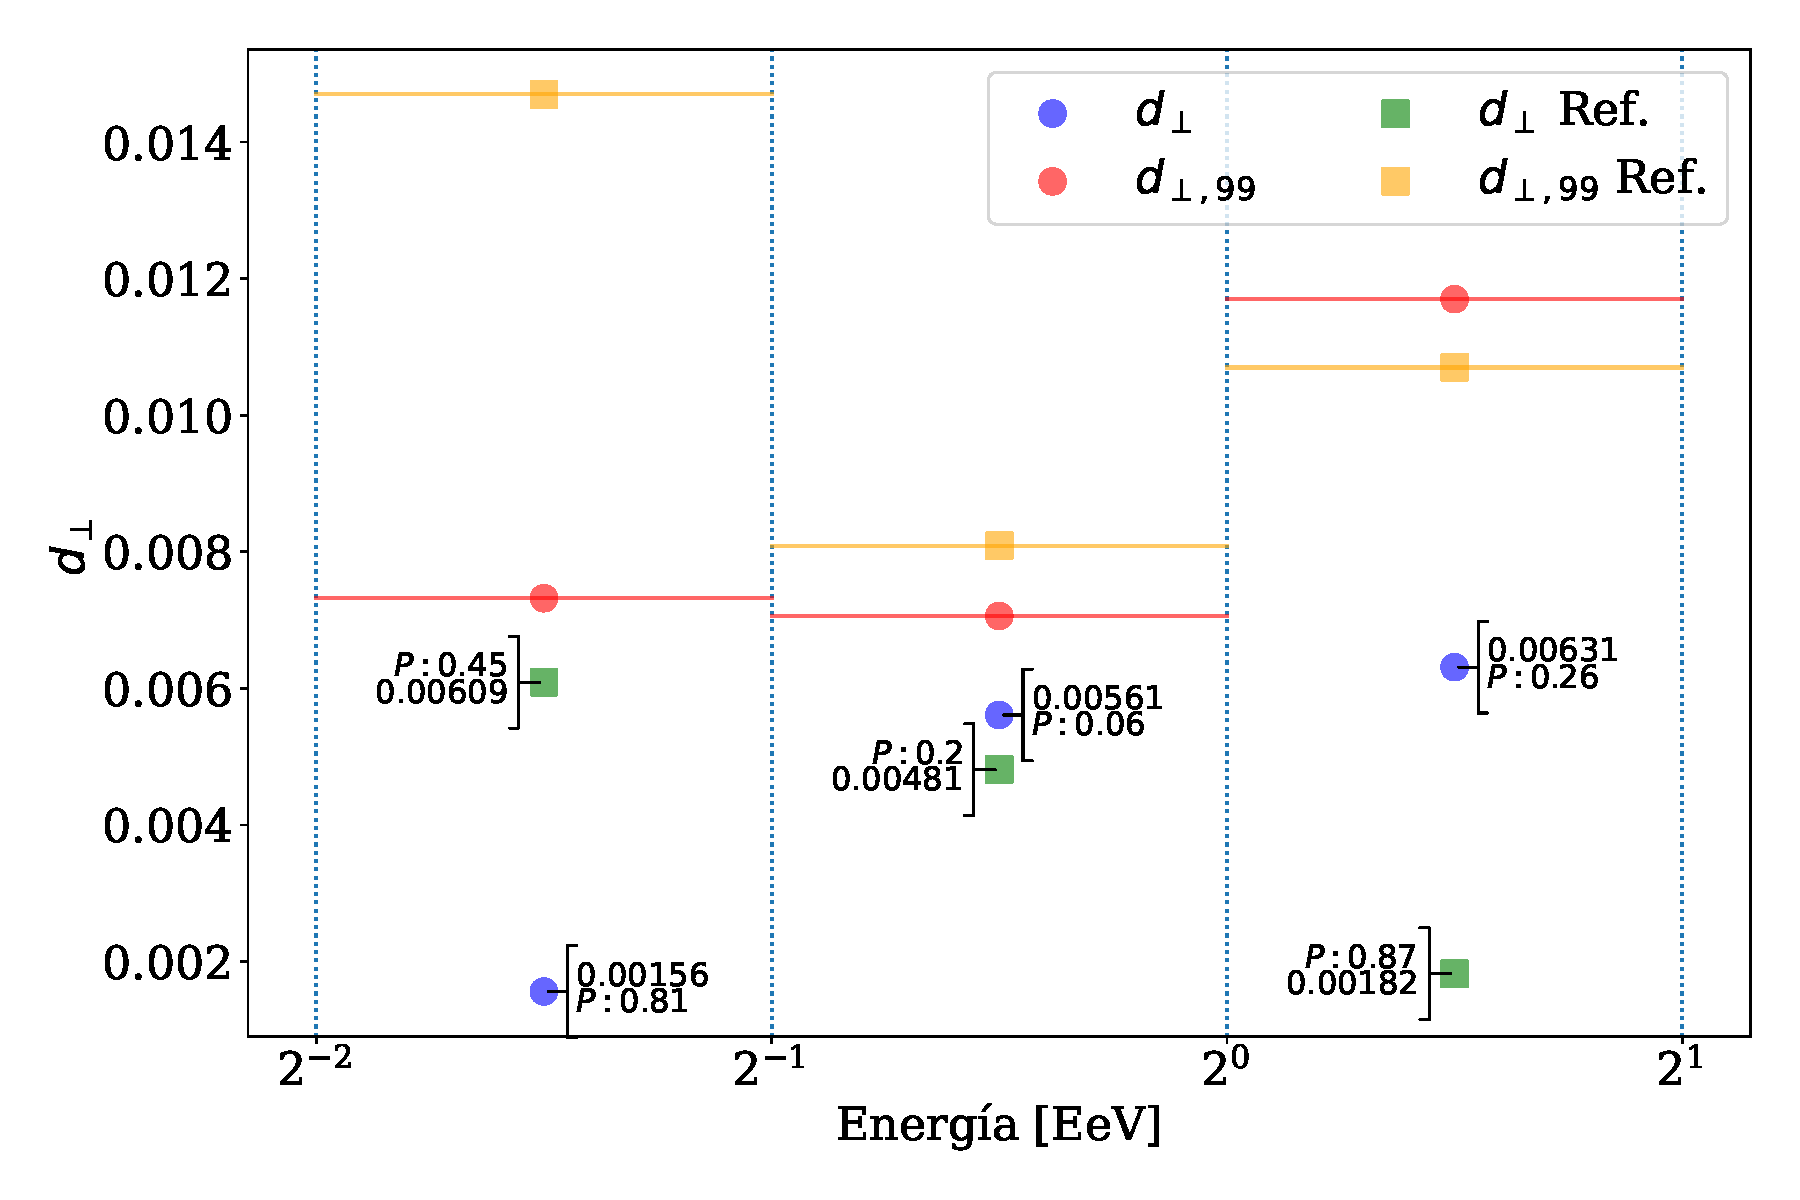
\includegraphics[width=0.75\textwidth]{d_perp_no_normalizado_v2.pdf}
            \end{center}
            \caption{Sin normalizar}
            \label{fig:no_normalizado}
        \end{small}
    \end{figure}
    
    Para compararlos mejor con respecto a $d_{\perp,UL}$, usamos el valor de cada rango y de cada conjunto de datos, para normalizar la amplitud de $d_{\perp,UL}$. Como se muestra en la Fig.\ref{fig:normalizado}, ahora $d_{\perp,UL}=1$ y los otros valores se pueden comparar. 

    \begin{figure}[H]
        \begin{small}
            \begin{center}
                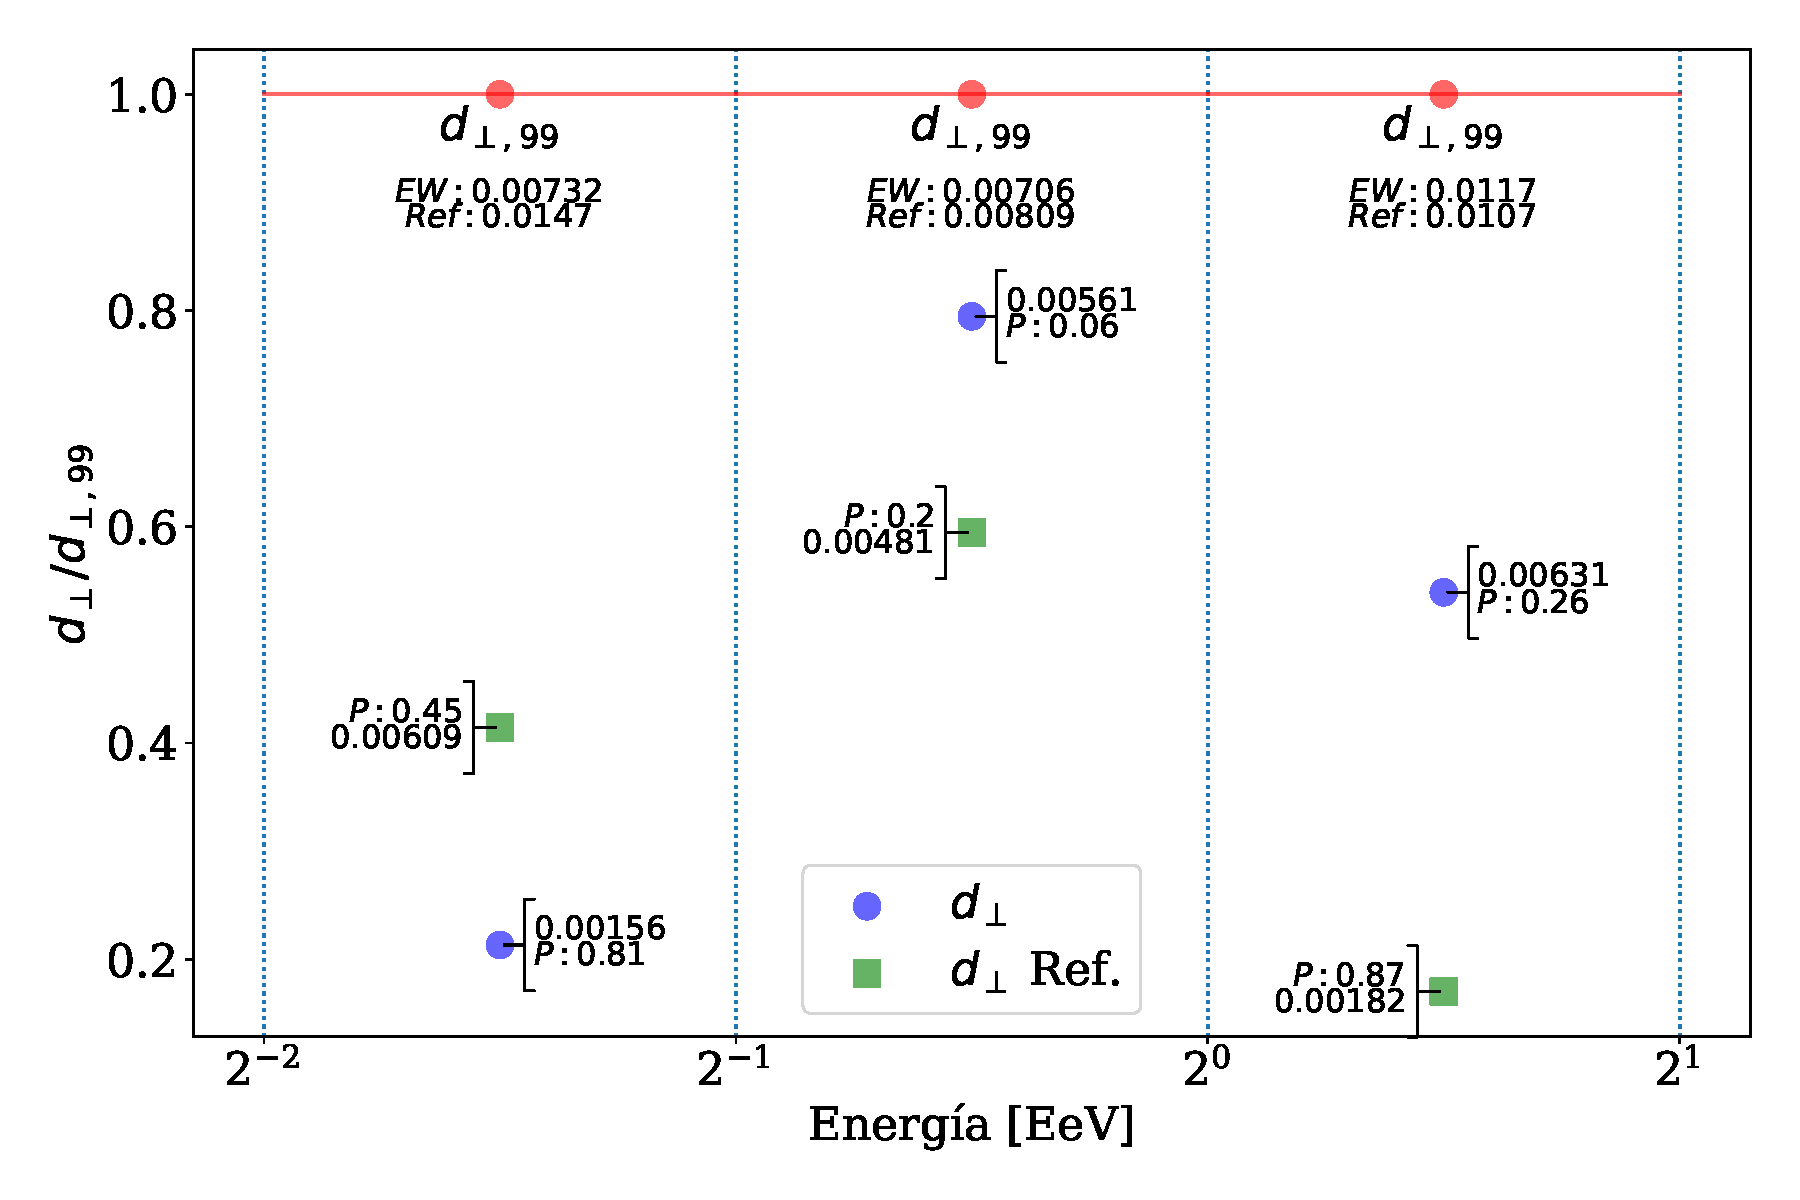
\includegraphics[width=0.75\textwidth]{d_perp_normalizado.pdf}
            \end{center}
            \caption{Valores normalizados con $d_{\perp,UL}$}
            \label{fig:normalizado}
        \end{small}
    \end{figure}

    También podemos comparar cuan apartados están con respecto al valor $\sigma_{x,y}$ y normalizar los valores en cada rango de energía, así se obtiene la Fig.\ref{fig:normalizado_sigma}.

    \begin{figure}[H]
        \begin{small}
            \begin{center}
                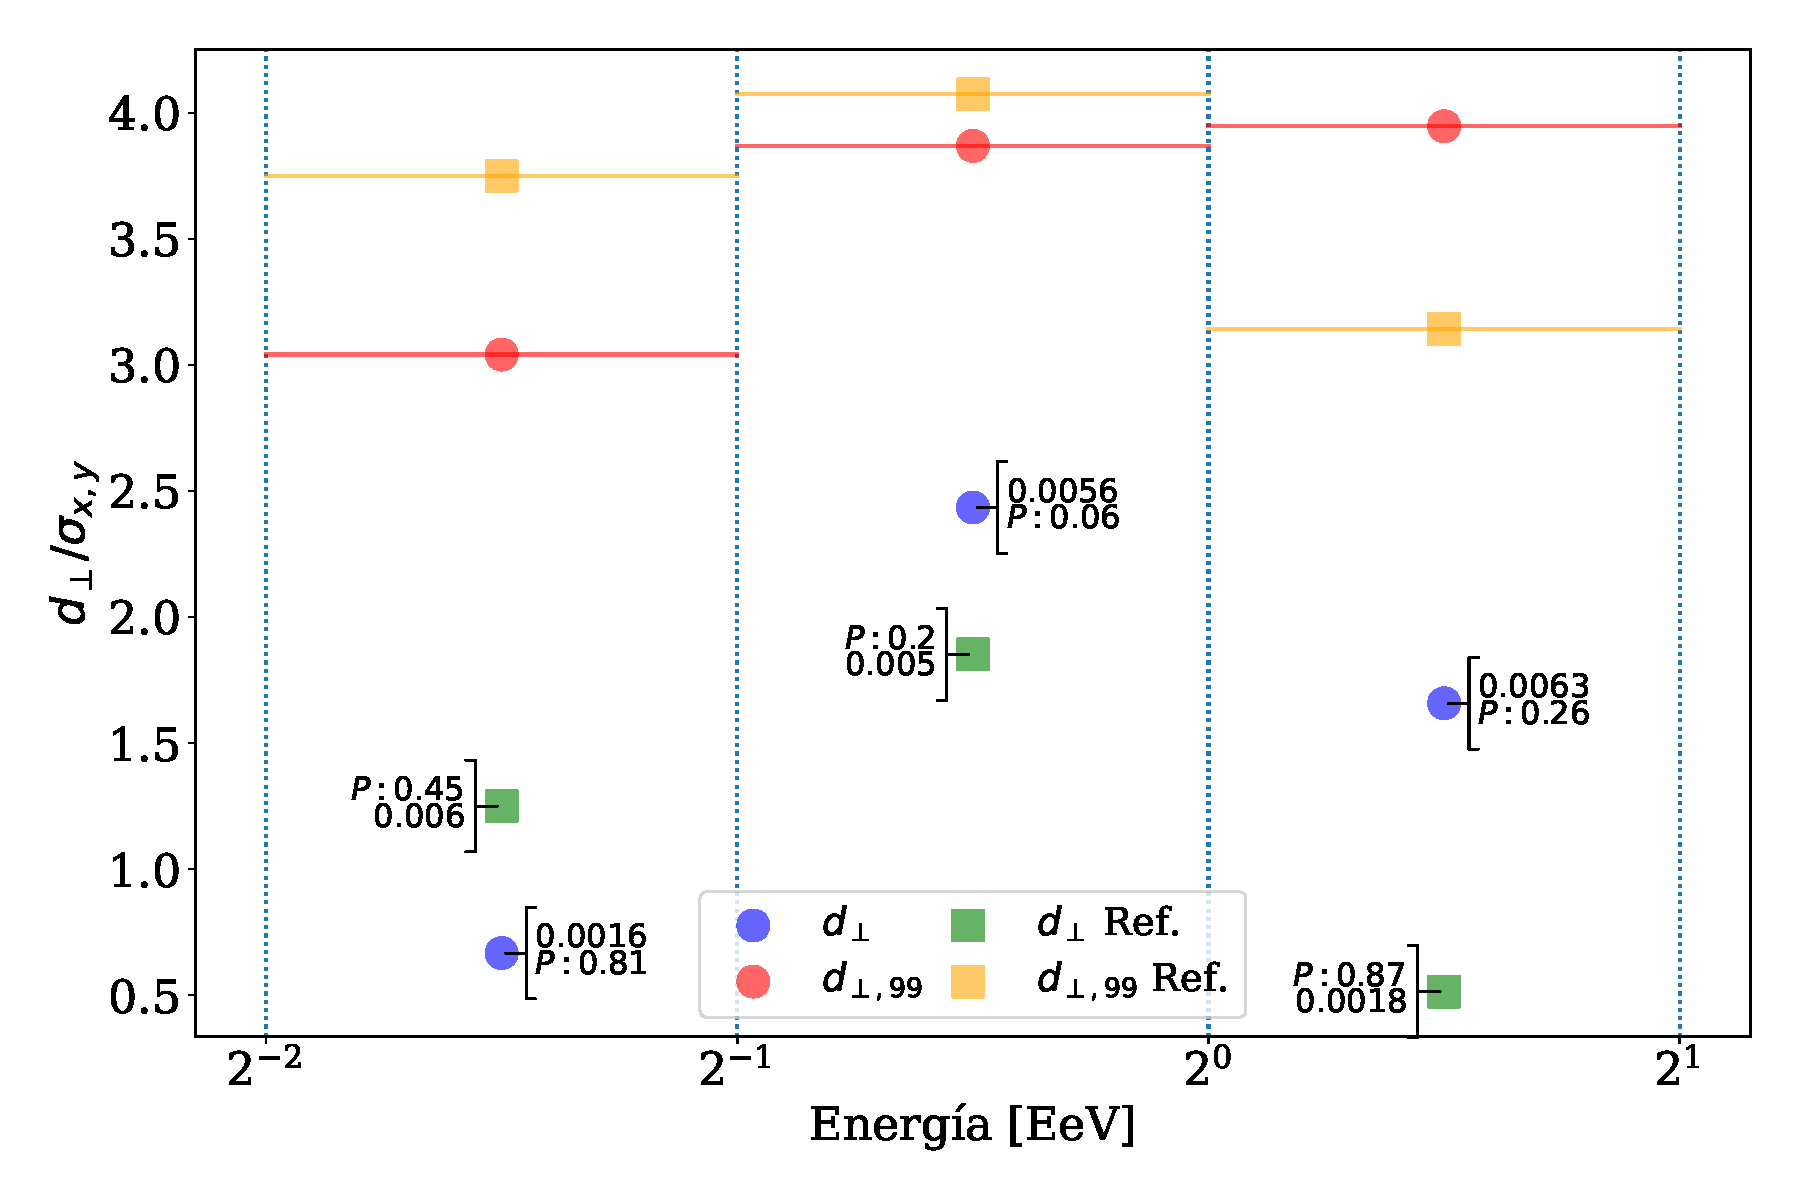
\includegraphics[width=0.75\textwidth]{d_perp_normalizado_sigmas_v4.pdf}
            \end{center}
            \caption{Valores normalizados con $d_{\perp,UL}$}
            \label{fig:normalizado_sigma}
        \end{small}
    \end{figure}

Por lo que ahora podemos decir que en los rangos entre 0.5 EeV - 1.0 EeV y 1.0 EeV - 2.0 EeV, la amplitud obtenida en este trabajo está por encima que la referencia. 

Para comparar los resultados en el  rango 0.25 EeV - 0.5 EeV, tenemos que tener en cuenta que el disparo estándar tiene una sensibilidad menor que el todos los disparos. Esto se ve claramente en la Tabla \ref{tab:}, donde el primer tiene 7 veces menos eventos para analizar. Por lo tanto, la discrepancia entre la referencia y los trabajos puede deberse a la  diferencia de eventos a estudiar causada por la sensibilidad del disparo.


Considerando los valores de $\sigma$ y $d_\perp$ para cada rango de energía, puedo comparar las direcciones, valores e incertidumbres en un sola figura como en la Fig.\ref{fig:incertidumbre}. Las líneas punteadas están centradas en los valores de referencia en cada rango de energía y con radio igual a sus incertidumbres. 

\begin{figure}[H]
    \begin{small}
        \begin{center}
            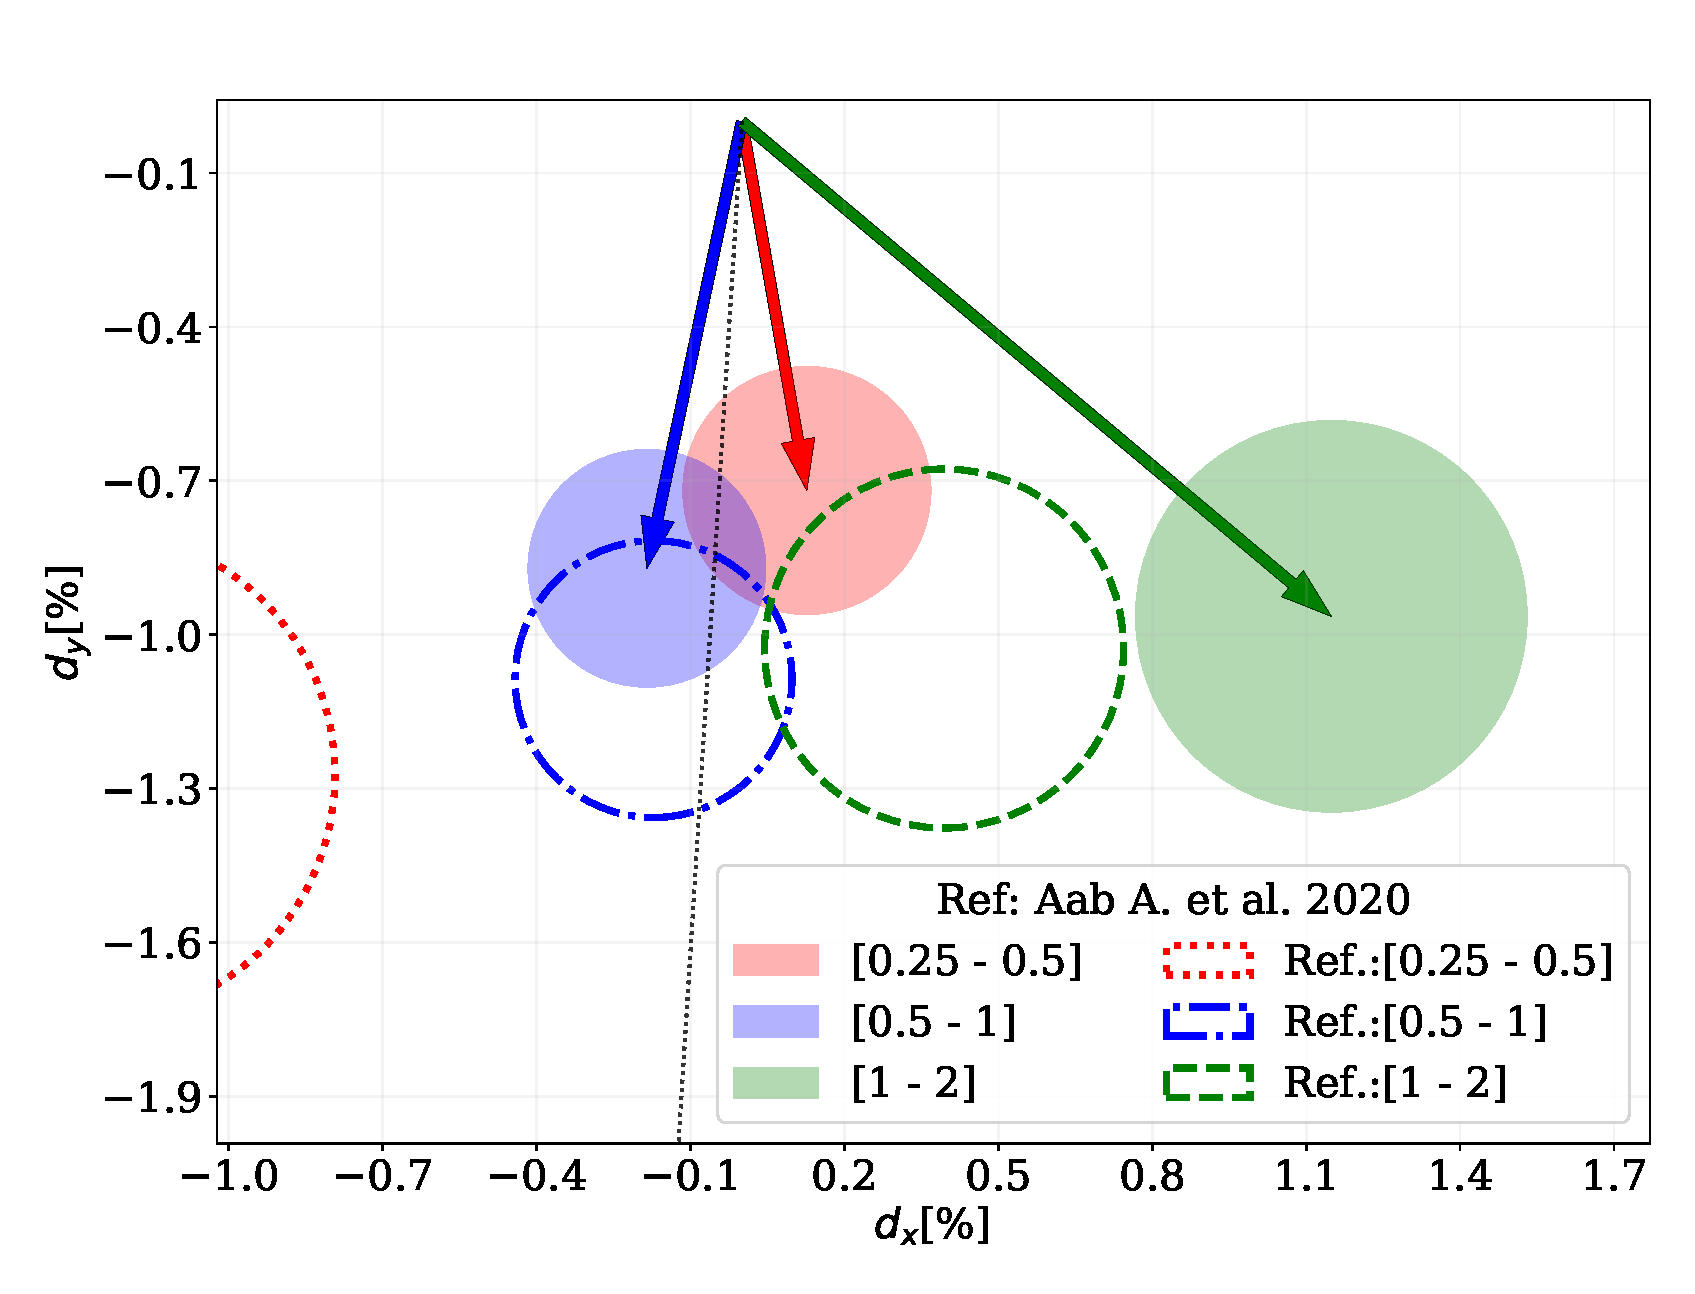
\includegraphics[width=0.75\textwidth]{comparando_sigmas_v2.pdf}
        \end{center}
        \caption{Amplitudes con incertidumbre, apuntando en la dirección  de la fase. Los círculos punteados los valores de referencia del trabajo \cite{Aab_2020} con sus respectivas incertidumbres y la línea punteada en negro marca la dirección del centro galáctico.}
        \label{fig:incertidumbre}
    \end{small}
\end{figure}


\section{Comparando resultados entre métodos para barridos de frecuencias}

\section{Verificación del código escrito durante la maestría}


\begin{table}[H]
    \begin{small}
        \begin{center}
            \begin{tabular}[c]{l|c|c|c|c|}
                                            & \multicolumn{4}{|c|}{2 EeV - 4 EeV}                                                               \\ \hline
                Frecuencia:                 & 366.25              & 366.25 (Sin pesos)  & 366.25 \cite{codigo}    & 366.25 \cite{Aab_2020}   \\ \hline
                Amplitud r [\%]:            & $0.5^{+0.3}_{-0.2}$ & $0.4^{+0.3}_{-0.2}$ & $0.5^{+0.3}_{-0.2}$     & -                          \\
                $r_{99}$ [\%]:              & 0.8                 & 0.8                 & 0.8                     & -                          \\\hline
                Amplitud $d_\perp$[\%]:     & $0.7^{+0.4}_{-0.2}$ & $0.5^{+0.4}_{-0.2}$ & $0.7^{+0.4}_{-0.2}$ 	  & $0.5^{+0.4}_{-0.2}$                    \\
                $d_{99}$ [\%]:              & 1.0                 & 1.0                 & 1.0                     & -                         \\
                $d_{\perp,UL}$[\%]:         & 1.9                 & 1.7                 & -                       & 1.4                               \\\hline
                $\sigma_{x,y}$[\%]:         & 0.34	              & 0.34	            & 0.34	                  & 0.34                           \\
                Probabilidad      :         & 0.14                & 0.33                & 0.15               	  & 0.34                       \\
                Fase[$^o$]:                 & 355$\pm$29          & 351$\pm$38          & 346$\pm$29              & 349$\pm$55                    \\
            \end{tabular}
        \end{center}
    \end{small}
    \caption{Características para las frecuencias solar y sidérea con el método Rayleigh en el primer armónico en el rango de energía 2 EeV - 4 EeV, obtenidos con el código de este trabajo aplicado al conjunto de datos de la referencia \cite{Aab_2020} y comparados con los resultados reportados en el último.}
\end{table}


\begin{table}[H]
    \begin{small}
        \begin{center}
            \begin{tabular}[c]{l|c|c||c|c|}
                                            & \multicolumn{2}{|c||}{8 EeV - 16 EeV}              & \multicolumn{2}{|c|}{16 EeV - 32 EeV}                   \\ \hline
                Frecuencia:                 & 366.25                    & 366.25 \cite{Aab_2020} & 366.25                   & 366.25 \cite{Aab_2020}   \\ \hline
                Amplitud r [\%]:            & $4.4^{+1.0}_{-0.8}$ 	    & -                      & $5.8^{+1.8}_{-1.3}$ 	    & -                         \\
                $r_{99}$ [\%]:              & 2.6                       & -                      & 4.9                      & -                          \\\hline
                Amplitud $d_\perp$[\%]:     & $5.6^{+1.2}_{-1.0}$ 	    & $5.6^{+1.2}_{-1.0}$    & $7.5^{+2.3}_{-1.8}$ 	    & $7.5^{+2.3}_{-1.8}$                   \\
                $d_{99}$ [\%]:              & 3.3                       & -                      & 6.3                      & -                         \\
                $d_{\perp,UL}$[\%]:         & 10                        & -                      & 16                       & -                                 \\\hline
                $\sigma_{x,y}$[\%]:         & 1.1	                    & 1.1                    & 2.1	                    & 2.1                           \\
                Probabilidad      :         & $2.3\times10^{-6}$	    & $2.3\times10^{-6}$     & $1.5\times10^{-3}$	    & $1.5\times10^{-3}$              \\
                Fase[$^o$]:                 & 96$\pm$11                 & 97$\pm$12              & 80$\pm$16                & 80$\pm$17                     \\
            \end{tabular}
        \end{center}
    \end{small}
    \caption{Características para las frecuencias solar y sidérea con el método Rayleigh en el primer armónico en distintos rangos de energía, obtenidos con el código de este trabajo aplicado al conjunto de datos de la referencia \cite{Aab_2020} y comparados con los resultados reportados en el último.}
\end{table}


\begin{biblio}
	\bibliography{mibib.bib}
\end{biblio}
    
    \end{document}
